% ============================================================
% UCRA -- Uncertainty-to-Reservation Closed-Loop Framework
% IEEE journal-style manuscript (IEEEtran, two-column)
%
% Build:  tectonic main.tex     (or pdflatex + bibtex + pdflatex x2)
% Figures: figures/*.png are the VERIFIED experiment outputs.
%          Boxes marked [PLACEHOLDER] are for the authors' own
%          diagrams -- drop your PDF/PNG in figures/ and replace
%          the \framebox with \includegraphics.
% ============================================================
\documentclass[journal]{IEEEtran}

\usepackage{graphicx}
\usepackage{amsmath,amssymb,amsfonts}
\usepackage{booktabs}
\usepackage{multirow}
\usepackage{array}
\usepackage{xcolor}
\usepackage[colorlinks=true,linkcolor=blue,citecolor=blue,urlcolor=blue]{hyperref}
\usepackage{url}

\graphicspath{{figures/}}

% ---------- placeholder helper for the authors' own diagrams ----------
\newcommand{\diagramplaceholder}[3]{%
  \begin{center}
    \fbox{\parbox[c][#1][c]{0.93\linewidth}{\centering
      {\large\bfseries [DIAGRAM PLACEHOLDER --- #2]}\\[6pt]
      {\itshape #3}\\[6pt]
      {\small Insert your diagram as \texttt{figures/#2.pdf} or
       \texttt{.png} and replace this box with
       \texttt{\textbackslash includegraphics\{#2\}}.}}}
  \end{center}}

% ---------- math shorthands ----------
\newtheorem{proposition}{Proposition}
\newcommand{\Rt}{R_t}
\newcommand{\D}{D}
\newcommand{\Dt}{D_t}
\newcommand{\uhat}{\hat{u}_t}
\newcommand{\spread}{\Delta_t}
\newcommand{\rhot}{\rho_t}

\newcommand{\qtau}{\hat{q}_{t,\tau}}

\begin{document}

\title{UCRA: Uncertainty-Aware Quantile Reservations for Self-Evolving
Resource Allocation in 5G Network Slicing}

\author{Tirumala~Sai~Kalyana~Madhur,
        Jadapola~Sai~Ganesh~Reddy,
        Sunkara~Ankit,
        Dhurbhakula~Dhanurdhar,
        and~Deepthi~Godavarthi%
\thanks{T.~S.~K.~Madhur, J.~S.~G.~Reddy, S.~Ankit, and
D.~Dhanurdhar are with the Department of Computer Science and
Engineering (B.Tech.\ undergraduate program).}%
\thanks{D.~Godavarthi is the project supervisor, Department of
Computer Science and Engineering
(e-mail: see Acknowledgment section).}%
\thanks{Code, configuration, and verified result artifacts for this
paper are available at the project repository
(\texttt{github.com/sai-ganesh-4539/UCRA}). The two datasets used are
publicly available on Zenodo (records 17815388 and 10610616).}}

\markboth{Uncertainty-Aware Quantile Reservations for 5G Network Slicing}%
{Madhur \MakeLowercase{\textit{et al.}}: UCRA}

\maketitle

\begin{abstract}
Network slicing promises logically isolated, service-tailored virtual
networks on shared 5G infrastructure, but its operation hinges on a
question that is usually answered crudely: how much capacity should a
slice reserve for the next interval when future demand is uncertain?
Over-reservation wastes spectrum that other tenants could monetize;
under-reservation violates service-level agreements and degrades
user experience. Existing approaches occupy two unattractive extremes:
static margins sized from peak historical load, which waste 30\% or
more of capacity, and end-to-end learned controllers, whose policies
are opaque, hard to audit, and brittle under distribution shift. This
paper presents UCRA (Uncertainty-to-Reservation Closed-Loop Resource
Allocation), a five-stage framework that turns calibrated probabilistic
demand forecasts into capacity reservations through an explicit,
auditable transform $\Rt = \qtau + \kappa\,\spread\,(1 + w\,\rhot)$,
where $\qtau$ is a deep quantile forecast, $\spread$ its dispersion,
$\rhot$ an online risk indicator, and $\kappa$ a single operator-facing
risk dial. A self-evolving stage detects drift from reservation
feedback and fine-tunes the forecaster on a reservoir replay buffer
under a formally causal information-flow protocol that we prove and
enforce in tests: the model can only learn from labels that would
already exist in a live deployment. On three weeks of live 5G/4G/2G
radio access network performance counters (302{,}052 records, 75
sectors), UCRA holds \textbf{0.0\% reservation violations at 72.1\%
utilization} and 10.7\% waste, where a peak-sized static reservation
wastes 30.5\%, a median-forecast policy violates 48.0\% of intervals,
and even a cheating oracle quantile still violates 16.3\%. A
three-seed study confirms stability (0.0\% violations in every seed;
utilization $67.6\%\pm3.4$). Under an injected $+35\%$ demand surge,
the causal self-evolving loop cuts post-surge violations by half
($34.3\%\pm5.9 \rightarrow 17.2\%\pm4.9$ across seeds) relative to a
frozen forecaster, while firing zero spurious updates on clean data. On
an independent CTTC 5G slicing workload (229 steady-state snapshots),
the same transform reduces slice reservation violations to 1.2--2.7\%
across URLLC, eMBB, and mMTC where the operator's default sizing
violates 5.8--43.7\%. The full pipeline --- data ingestion, training,
closed-loop evaluation, leakage audit, and three-seed verification ---
is open and reproducible from the accompanying repository.
\end{abstract}

\begin{IEEEkeywords}
5G network slicing, resource reservation, quantile regression, deep
learning, uncertainty quantification, online learning, concept drift,
replay buffers, risk management, reproducibility.
\end{IEEEkeywords}

\section{Introduction}
\label{sec:intro}

\IEEEPARstart{5}{G} network slicing is one of the defining operational
ideas of modern mobile networks: a single physical radio access and
transport infrastructure is carved into logically isolated virtual
networks, each engineered for a service class with its own key
performance indicators --- ultra-reliable low-latency communications
(URLLC), enhanced mobile broadband (eMBB), and massive machine-type
communications (mMTC)~\cite{rost2017network,afolabi2018slicing}.
The economic promise of slicing rests on a deceptively simple
operational primitive: the operator periodically decides how much of a
shared resource pool (radio spectrum, transport bandwidth, compute) to
\emph{reserve} for each slice or sector over the next control interval.
Every downstream commitment --- a guaranteed bitrate for an industrial
URLLC flow, a busy-hour throughput target for a video eMBB cohort ---
is ultimately backed by that reservation decision. When the reservation
meets or exceeds realized demand, users are served and the SLA holds;
when it falls short, the slice violates its contract; whatever is
reserved but unused is idle capital that neighboring tenants cannot
use.

The difficulty is that the reservation must be committed \emph{before}
demand realizes. Mobile traffic is strongly periodic (diurnal and
weekly cycles), heavy-tailed at 15-minute granularity, and subject to
abrupt regime shifts --- mass events, flash crowds, application
launches, holidays --- that no historical model fully
anticipates~\cite{shafiq2012cellular,sciancalepore2017mobile}. A reservation
policy is therefore an exercise in decision-making under uncertainty,
and the natural language for that exercise is probabilistic
forecasting: predict not a single demand number but a distribution, and
size the reservation from a calibrated upper quantile of that
distribution. Yet the majority of deployed practice still sizes
reservations from static rules of thumb --- peak-plus-margin being the
most common --- precisely because the probabilistic alternative has
been perceived as operationally fragile.

This paper argues that the perception is outdated, and that the
remaining fragility has a different root: not the quality of deep
probabilistic forecasts, which is now adequate, but the
\emph{interface} between forecasts and reservations, and the
\emph{information hygiene} of the learning loop that adapts them. We
present UCRA, a closed-loop framework that makes both explicit. UCRA
comprises five stages: (1) a quantile LSTM forecaster that emits a
full predictive distribution of demand one hour ahead; (2) an
\emph{uncertainty-to-reservation transform} $\Phi$ that converts the
forecast distribution into a reservation target through one auditable
equation with a single interpretable risk parameter $\kappa$; (3) a
risk-adaptive allocation that distributes an aggregate reservation
across competing sectors or slices in proportion to demand pressure
and risk; (4) an update-and-release mechanism with EWMA smoothing and
release hysteresis that suppresses reservation churn; and (5) a
self-evolving learning stage that watches the reservation feedback
stream (violations, demand z-scores), detects distribution drift, and
fine-tunes the forecaster on a reservoir-sampled replay buffer ---
under an information-flow protocol that guarantees the loop never
learns from labels a live system could not yet possess.

\subsection{Motivation: two failure modes of the obvious designs}

The two canonical baselines fail in instructive, opposite directions,
and our experiments quantify both on real data. A \emph{static
peak-plus-margin} reservation --- the historical maximum demand, held
constant --- never violates on our three-week evaluation window, but
wastes 30.5\% of capacity; on a three-week trace that is roughly a
week of capacity paid for and never used. Worse, its safety is
conditional on stationarity: had a single test-window spike exceeded
the training peak, the ``safe'' policy would have violated with no
recourse. A \emph{median-forecast} reservation --- reserve what the
point forecast says demand will be --- is the opposite failure: it
tracks demand tightly (its mean absolute tracking error is the lowest
of all policies we test) yet violates the reservation in 48.0\% of
15-minute intervals on the same window, because the median of a
right-skewed distribution is by construction exceeded half the time.
The lesson is structural: violation rate and utilization trade off
along a frontier, and the frontier's shape is determined by how
uncertainty information enters the reservation rule. UCRA's
contribution is to make that entry point explicit, tunable, and
adaptive.

\subsection{Motivation: leakage is the silent killer of online-learning claims}

Self-evolving (continually learning) forecasters are increasingly
proposed for network operations, and our own Stage~5 is one. But
online-learning experiments carry a methodological trap that is easy
to fall into and easy to miss: at loop time $t$ a forecaster that
predicts an $H$-step horizon holds labels only for slots up to $t$;
its multi-step training targets for slots $t+1,\dots,t+H-1$ do not
\emph{exist} yet. An evaluation harness that stores full multi-step
windows into a replay buffer at time $t$ --- as ours originally did
--- lets the fine-tuned model peek as much as $H-1$ slots into the
future, inflating post-adaptation performance in a way that no live
deployment could realize. The pre-submission audit of this paper
caught exactly this flaw in our own pipeline; the final version
therefore introduces \emph{delayed causal replay}, which admits a
training window into the buffer only when its last label has been
observed, and refreshes forecasts only for slots whose reservations
have not yet been committed. We formalize the rule, prove its
sufficiency, unit-test it, and re-run every experiment under it. We
highlight this not as a detail but as a reusable evaluation protocol
for the growing literature on self-adaptive network
controllers~\cite{kapoor2023leakage}.

\subsection{A running example}

To make the framework concrete before the formal treatment, consider
one operational day on the evaluated network. At 05:45 the forecast
for the 06:00 slot reads a median of 61{,}200 with a wide
morning-ramp dispersion of 12{,}400; the transform reserves
$\approx$77{,}500 --- well above the median, because the forecaster
itself reports high uncertainty about how fast the morning ramp will
run. At 13:30, demand is stable and the band tightens; the same
formula reserves barely 6\% above the base quantile. At 21:00 a
flash crowd begins: reservations start violating, the rolling
violation indicator rises, the risk term inflates every buffer by up
to 45\% within its bounded range, and if the surge persists past the
drift trigger the forecaster is fine-tuned --- on strictly past
labels only --- so the next morning's forecasts reflect the new
regime. Every one of these decisions is a four-term arithmetic
expression an operator can audit after the fact, and the paper's
central empirical claim is that this loop, so specified, held zero
violations for three weeks of live traffic at two-thirds utilization
while static sizing wasted nearly a third of capacity.

\subsection{Contributions}

This paper makes the following contributions:

\begin{enumerate}
\item \textbf{An auditable uncertainty-to-reservation transform.} A
closed-form mapping $\Phi$ from a quantile forecast to a reservation,
$\Rt = \qtau + \kappa\,\spread\,(1 + w\,\rhot)$, with clamping to
a minimum-headroom floor and a capacity ceiling. One dial, $\kappa$,
moves the operator along the risk--utilization frontier; we trace the
full frontier empirically.
\item \textbf{A five-stage closed loop with self-evolution.} Quantile
LSTM forecasting, risk-feedback state, reservation smoothing with
release hysteresis, and trigger-based continual learning from a
reservoir replay buffer, wired into one control loop with per-slot
feedback.
\item \textbf{A formally causal online-learning protocol.} The
delayed replay intake (admission at $t+H-1$) and partial forecast
refresh (only slots $>t$), with a sufficiency argument, unit tests
that fail on the leaky variant, and a head-to-head quantification
showing the leaky variant inflates adaptation gains.
\item \textbf{A verified, multi-dataset empirical study.} On live RAN
performance counters: 0.0\% violations at 72.1\% utilization (seed
42; $67.6\%\pm3.4$ across three seeds) versus 30.5\% waste for static
peak sizing and 48.0\% violations for median-forecast sizing; a
cheating oracle still violates 16.3\%. Under a $+35\%$ surge: causal
self-evolution halves post-surge violations ($34.3\%\pm5.9
\rightarrow 17.2\%\pm4.9$). On the independent CTTC slicing workload:
1.2--2.7\% slice violations versus 5.8--43.7\% for the operator's
default sizing.
\item \textbf{An honest negative-control analysis.} The clean RAN
window triggers \emph{zero} self-evolution updates in all seeds: the
drift detector disciplines itself when there is nothing to fix. We
report this as a false-positive control and scope all online-learning
claims to the drift experiment, rather than over-claiming from the
clean run.
\item \textbf{Full reproducibility.} Deterministic configurations,
pinned datasets (Zenodo), unit tests including causality regression
tests, and one-command reruns of every table and figure in this
paper.
\end{enumerate}

\subsection{Paper organization}

Section~\ref{sec:related} reviews related work on slicing resource
management, predictive uncertainty, and online adaptation.
Section~\ref{sec:novelty} states the novelty claims and their
relationship to prior art. Section~\ref{sec:system} formalizes the
system model and the reservation problem. Section~\ref{sec:method}
details the five stages, including the causal replay protocol.
Section~\ref{sec:setup} describes datasets, baselines, metrics, and
the verification protocol. Section~\ref{sec:results} presents the
verified results. Section~\ref{sec:discussion} discusses scope,
limitations, and threats to validity, and Section~\ref{sec:conclusion}
concludes.

\section{Related Work}
\label{sec:related}

\subsection{Network Slicing and Resource Allocation}

Network slicing has been studied extensively since its
standardization in 5G, from architecture
frameworks~\cite{rost2017network,afolabi2018slicing} to
orchestration and lifecycle management~\cite{foukas2017networking}.
Resource allocation for slices spans a wide methodological spectrum.
At the static end, operators size slices from engineering rules and
peak-load studies; these approaches are transparent and stable but
cannot track demand dynamics, and empirical studies repeatedly report
substantial over-provisioning as the price of
SLA safety~\cite{sciancalepore2017mobile}. At the dynamic end,
optimization-based approaches formulate slice embedding, scaling, or
admission as integer programs solved on rolling
horizons~\cite{yu2008rethinking}, and learning-based approaches
train reinforcement-learning agents to adjust slice resources from
feedback~\cite{wang2017intelligent,bega2019deepcog}. RL-based slice controllers
can in principle discover policies beyond human design, but they
raise adoption barriers that this paper takes seriously: the policy
is a black box whose failure modes are hard to audit, the training is
sample-hungry on infrastructure where exploration is costly, and the
learned controller is notoriously sensitive to distribution shift.
UCRA deliberately positions itself between the extremes: the forecast
is learned, but the decision layer is a single closed-form transform
that an operator can read, clamp, and reason about, in the spirit of
interpretable control for safety-critical
infrastructure~\cite{rudin2019stop}.

\subsection{Demand Prediction for Network Operations}

Traffic prediction has a long history in networking, from
classical time-series models~\cite{box2015time} to deep sequence
models. Recurrent architectures, and LSTMs in
particular~\cite{hochreiter1997lstm}, remain strong, well-understood
baselines for 15-minute to hourly network demand forecasting, with
convolutional and attention alternatives offering accuracy gains on
dense multivariate settings~\cite{zhang2017deep}. Applications
include cellular traffic forecasting for proactive
scaling~\cite{zhang2019transfer}, capacity planning, and anomaly
detection. Point forecasts, however, answer only part of the
reservation question: committing capacity requires knowing how wrong
the forecast can be. Probabilistic alternatives include Bayesian
neural networks~\cite{gal2016dropout}, deep ensembles, and --- most
directly relevant here --- \emph{quantile regression}, which trains a
model to output several conditional quantiles simultaneously by
minimizing the pinball (quantile) loss~\cite{koenker1978regression}.
Quantile forecasts are standard in electricity markets and load
serving~\cite{hong2016probabilistic} precisely because planners must
commit resources against uncertain demand, and we import that
tradition into slicing. Calibration --- whether the nominal 90\%
interval actually covers ~90\% of outcomes --- is the property that
makes such forecasts decision-grade, and we measure it explicitly
(Section~\ref{sec:results-calibration}).

\subsection{From Forecasts to Actions: Predictive Resource Management}

Converting predictive uncertainty into resource decisions has been
explored in cloud and network contexts. Forecast-driven autoscaling
sizes server fleets from predicted load, with queueing-theoretic
headroom rules~\cite{gandhi2012autoscale};
probabilistic variants size from predicted demand
distributions~\cite{ islam2012provisioning}. In wireless networks,
predictive resource allocation uses traffic forecasts to pre-allocate
PRBs, pre-warm carriers, or schedule sleep states. Closest in spirit
to UCRA, measurement-based admission control sized capacity from
recent traffic statistics with robustness
guarantees~\cite{grossglauser1999adaptive}.
Three gaps remain. First, most of this literature treats the
forecast-to-action mapping as a fixed engineering constant (a safety
factor), losing the connection between the operator's risk appetite
and the frontier position. Second, the risk feedback loop --- using
recent reservation outcomes to modulate the buffer --- is usually
absent. Third, the evaluation rarely closes the loop: metrics are
computed on forecast accuracy (pinball loss, coverage) rather than on
the operational reservation outcomes (violations, utilization, waste)
that the deployment actually cares about. UCRA addresses all three:
$\Phi$ exposes a single risk dial $\kappa$ whose frontier we trace
empirically; the risk indicator $\rhot$ closes the feedback loop
inside the transform; and all reported metrics are closed-loop
reservation outcomes on held-out windows.

\subsection{Drift Detection and Continual Learning}

Distribution shift is the normal condition of production networks:
traffic mix evolves, events recur, application behavior changes.
Drift detection is a mature field --- sequential tests such as
Page's CUSUM and the Page--Hinkley test~\cite{page1954continuous},
ADWIN's adaptive windowing~\cite{bifet2007learning}, and
population-stability statistics are standard tools. On detection,
continual-learning methods update the model without erasing prior
competence; experience replay is the simplest and most robust family,
and reservoir sampling~\cite{vitter1985random} maintains a uniform
sample of history in a fixed-size buffer, which directly mitigates
catastrophic forgetting~\cite{chaudhry2019continual,rolnick2019experience}.
UCRA's Stage~5 combines a dual-trigger monitor (rolling reservation
violation rate OR demand z-score) with reservoir replay and gentle
fine-tuning. What is novel is not the ingredients but the
\emph{contract}: a formally stated information-flow rule for what the
updater is allowed to know, enforced in code and tested, motivated by
the observation that online-learning evaluations routinely --- and
often unknowingly --- grant the learner access to labels that do not
yet exist, a special case of the leakage taxonomy of
Kapoor and Narayanan~\cite{kapoor2023leakage}. Prequential
evaluation~\cite{dawid1984present} formalizes the honest variant:
predict-then-observe in strict temporal order; our protocol is the
multi-step-horizon generalization of that principle for replay-based
updaters.

\subsection{Positioning Against Learned Slice Controllers}

The closest learned-controller line of work is DeepCog
\cite{bega2019deepcog}, which trains a deep network to output slice
capacity demand forecasts that a downstream optimizer converts into
slicing decisions, reporting large gains in resource efficiency on
synthetic and emulated topologies; mobile-traffic-forecast-driven
slicing utilization was likewise analyzed by Sciancalepore et
al.~\cite{sciancalepore2017mobile}. UCRA differs in three deliberate
ways. First, the forecast is \emph{probabilistic} (a full quantile
vector) rather than a point estimate, so the uncertainty the decision
layer must absorb is measured, not assumed. Second, the
decision layer is an explicit equation with one risk parameter rather
than a learned policy or an optimizer over a learned model --- weaker
in raw fitting power, stronger in auditability, and immune to the
distribution-shift brittleness that end-to-end controllers exhibit.
Third, UCRA's evaluation protocol holds the \emph{online-learning
component} to a causal information-flow contract
(Section~\ref{sec:stage5}); learned-controller evaluations, including
ours originally, rarely do, and Section~\ref{sec:leakage-audit}
quantifies what that omission was worth in our own pipeline.

\subsection{Uncertainty-Aware Provisioning in Adjacent Domains}

The pattern that UCRA instantiates --- forecast a distribution, then
commit a resource against a chosen quantile with an explicit risk
dial --- is mature in adjacent domains, and the borrowings are
deliberate. In electricity systems, probabilistic load forecasting
has fed unit commitment and reserve sizing for a decade: system
operators procure spinning reserve against forecast quantiles, and
the literature treats calibration as a procurement-relevant property
exactly as we treat coverage here~\cite{hong2016probabilistic}. In
cloud capacity management, AutoScale provisions server tiers from
predicted load with robustness margins and switching-cost
awareness~\cite{gandhi2012autoscale} --- the direct ancestor of our
Stage~4 smoothing and release hysteresis --- and empirical
provisioning models forecast workload to adapt resource
allocations~\cite{islam2012provisioning}. Measurement-based admission
control established the principle of committing capacity from
recent traffic statistics with robustness
guarantees~\cite{grossglauser1999adaptive}. What the slicing domain
has lacked is the assembly: these ingredients (calibrated
conditional quantiles, a priced buffer, feedback modulation,
churn-bounded actuation, and honest online adaptation) exist
separately, but no slicing resource manager composes them into one
auditable loop, evaluated closed-loop on live network data. That
composition is UCRA's contribution, and the adjacent-domain
literature provides the confidence that each ingredient is sound.

\subsection{Datasets and Reproducibility in 5G Research}

Progress in this area depends on public, realistic datasets. The CTTC
B5G slicing dataset~\cite{farreras2024cttc} provides steady-state
slicing simulation snapshots with per-slice reservations, offered
traffic, and QoS outcomes; the live RAN performance-counter
dataset of Lehoczky et al.~\cite{lehoczky2026ran} provides three
weeks of 15-minute sector-level 5G/4G/2G counters from an operational
network. Both are on Zenodo with stable identifiers and are used
here. Reproducibility has become a pressing concern for ML-for-networks
research~\cite{pineau2021improving}; UCRA releases its full pipeline
--- ingestion, training, closed-loop evaluation, causality unit
tests, and the three-seed verification driver --- with pinned
configuration files so that every number in Section~\ref{sec:results}
can be regenerated from a clean clone.

\section{Novelty and Contributions}
\label{sec:novelty}

This section states precisely what is new in UCRA relative to the
prior art surveyed in Section~\ref{sec:related}, and what is
deliberately \emph{not} claimed. We organize the novelty into five
claims, each paired with the evidence that supports it in
Section~\ref{sec:results}.

\subsection{Claim 1: A single-equation, operator-auditable
uncertainty-to-reservation transform}

Prior forecast-driven provisioning either buries the uncertainty
inside a learned policy (RL agents, end-to-end neural controllers) or
uses fixed engineering factors disconnected from the forecast's own
uncertainty estimate. UCRA's transform $\Phi$ (Eq.~\eqref{eq:phi}) is,
to our knowledge, the first slicing reservation rule that (i) consumes
the forecast distribution directly (a quantile and its dispersion),
(ii) modulates the buffer by an online risk indicator computed from
reservation feedback, and (iii) exposes exactly one interpretable
parameter $\kappa$ whose effect traces a measurable risk--utilization
frontier (Fig.~\ref{fig:kappa}). The transform is auditable in the
strong sense of Rudin~\cite{rudin2019stop}: given any reservation
decision, the operator can decompose it into forecast, uncertainty,
risk, and policy terms in seconds.

\subsection{Claim 2: Closed-loop coupling with churn suppression}

Stage~4's update rule couples the reservation target to realized
demand through EWMA smoothing plus \emph{release hysteresis}: slack is
released only after sustained non-use. On real 15-minute RAN data this
combination yields reservations that track demand (10.7\% tracking
error) while never violating, and it suppresses the oscillation that
naive target-chasing produces on bursty traffic. The combination of
probabilistic targets, hysteresis-bounded actuation, and per-slot
feedback into both the transform and the drift monitor is, to our
knowledge, not present as a unit in prior slicing resource managers.

\subsection{Claim 3: A formally causal protocol for online-learning
evaluation}

The self-evolution stage is architecturally conventional (drift
trigger + reservoir replay + fine-tuning); the novelty is the
evaluation contract. We formalize \emph{causal label availability} for
multi-step forecasters: a window observed at time $t$ with horizon
$H$ may enter the training pool no earlier than $t+H-1$
(Proposition~\ref{prop:causal}), and a model update at time $t$ may
only alter forecasts for slots later than $t$. We are not aware of
prior slicing-reservation work that states, enforces, and unit-tests
this contract. The practical significance is demonstrated
empirically: the leaky variant of our own pipeline inflates the
apparent benefit of self-evolution, and the corrected protocol still
supports the qualitative claim (halved post-surge violations) with
defensible numbers. We offer the protocol as a reusable standard for
evaluating self-adaptive network controllers, complementary to the
general leakage taxonomy of Kapoor and Narayanan~\cite{kapoor2023leakage}.

\subsection{Claim 4: Trigger discipline as a first-class result}

Self-evolving systems are usually evaluated only on scenarios where
adaptation helps. UCRA is evaluated symmetrically. On the clean RAN
window --- three weeks of live traffic --- the drift triggers fire
\emph{zero} times in every seed while the system holds 0.0\%
violations: the insurance policy is armed but never cashed, and never
fires spuriously. On the surged window the same triggers fire
reliably and adapt. This symmetric evidence (silence when unneeded,
action when needed) is, we argue, the correct standard for
evaluating trigger-based adaptivity, and it is rarely reported.

\subsection{Claim 5: Verified reproducibility as a methodological
contribution}

Every headline number in this paper is regenerated by a scripted
pipeline from pinned public datasets, with configuration-controlled
seeds, a three-seed verification driver, causality regression tests,
and an explicit leakage audit (Section~\ref{sec:leakage-audit}).
During preparation, the audit invalidated two of our own earlier
results (the replay leakage above, and an outcome-informed risk term
in the CTTC evaluation), which we document and correct in the final
version. We consider the audit methodology --- treat your own
information flows as adversarially reviewable --- a contribution in
its own right for the ML-for-networking community, where evaluation
subtleties are easy to miss and expensive to discover post
publication.

\subsection{What we do not claim}

UCRA does not claim a novel forecaster: the quantile LSTM is a
deliberately standard, well-understood architecture
(Section~\ref{sec:stage1}), and forecast accuracy is treated as a
solved-enough subproblem. We do not claim optimality of $\kappa$; the
frontier (Fig.~\ref{fig:kappa}) is presented so each operator can
choose. We do not claim the CTTC risk-modulation term is decisive ---
on that dataset the honest finding is that it is not
(Section~\ref{sec:results-cttc}), and we say so. Finally, we do not
claim generality beyond the evaluated regimes; threats to validity
are cataloged in Section~\ref{sec:discussion}.

\section{System Model and Problem Formulation}
\label{sec:system}

\subsection{Network and Slicing Model}

We consider an operator infrastructure divided into a set of
\emph{reservable pools} --- a radio access network partitioned into
sectors, or a slicing-enabled transport/compute fabric partitioned
into slices. Time is slotted at the operational control granularity
$\delta$; throughout this paper $\delta = 15$ minutes, the standard
PM-counter granularity of 3GPP performance management and of our
dataset. Each pool $i$ has a physical capacity $C_i$: the maximum
demand it can serve in one slot. The aggregate demand offered to pool
$i$ in slot $t$ is $\Dt^{(i)} \ge 0$, a realization of a stochastic
process with strong diurnal and weekly seasonality, heavy-tailed
within-slot bursts, and occasional regime shifts
(mass events, flash crowds, gradual traffic evolution).

At each slot $t$ the controller commits a \emph{reservation}
$\Rt^{(i)} \in [0, C_i]$ for pool $i$ covering slot $t+1$. The
reservation is a hard commitment in the operational sense: demand up
to $\Rt$ is served with contracted quality; demand beyond $\Rt$
violates the SLA (blocked, degraded, or served from best-effort
overflow at a quality penalty). Reservations may be revised every
slot, but large swings are themselves costly --- reconfiguration
signaling, spectrum map churn, and upstream commitment churn --- which
we model with a switching penalty implicitly smoothed by the update
mechanism of Section~\ref{sec:stage4}.

\subsection{Closed-Loop Decision Process}

The controller observes, at the end of slot $t$: the demand history
$\{\D_{t-k}\}_{k=0}^{K-1}$ (a window of $K$ past slots; $K=96$, i.e.,
24 hours), the realized outcome of past reservations
$\mathbf{1}[\D_{t} > R_{t}]$, and auxiliary feedback (recent
violation rate, demand level relative to training statistics). It
does \emph{not} observe $\D_{t+1}, \D_{t+2}, \dots$. This is the
defining constraint of the problem and, as
Section~\ref{sec:leakage-audit} details, the constraint most often
violated inadvertently in experimental harnesses. Formally, the
information set available when choosing $R_{t+1}$ is
\begin{equation}
\mathcal{F}_t \;=\; \sigma\bigl(\D_{t-K+1..t},\;
\{R_{s}\}_{s\le t},\; \{\mathbf{1}[\D_s > R_s]\}_{s \le t}\bigr),
\label{eq:filtration}
\end{equation}
and any admissible policy must be $\mathcal{F}_t$-measurable. All
components of UCRA --- the forecaster, the transform, the risk state,
the replay buffer --- are functions of $\mathcal{F}_t$ only; the unit
tests of Section~\ref{sec:setup} enforce this mechanically.

\subsection{Reservation Metrics}

For a pool with capacity $C$ and a reservation trajectory
$\{R_t\}_{t=1}^{T}$ against realized demand $\{\D_t\}_{t=1}^{T}$,
we use four closed-loop metrics.

\emph{Violation rate} (risk exposure):
\begin{equation}
V \;=\; \frac{1}{T}\sum_{t=1}^{T} \mathbf{1}[\D_t > R_t].
\label{eq:violation}
\end{equation}
This is the SLA-failure frequency --- the quantity the operator is
contractually penalized for.

\emph{Utilization} (efficiency of the committed capacity):
\begin{equation}
U \;=\; \frac{1}{T}\sum_{t=1}^{T} \min\!\left(\frac{\D_t}{R_t},\,1\right).
\label{eq:utilization}
\end{equation}
Per-slot utilization is capped at 1: over-demand does not inflate
utilization; it appears as violations instead. A policy can therefore
exhibit both high utilization and high violation rate
(median-forecast policies do exactly this on our data).

\emph{Waste} (idle committed capacity):
\begin{equation}
W \;=\; \frac{1}{T\,C}\sum_{t=1}^{T} \max(R_t - \D_t,\, 0),
\label{eq:waste}
\end{equation}
the fraction of physical capacity that was reserved, went unused, and
could have been monetized by other tenants.

\emph{Reservation error} (tracking):
\begin{equation}
E \;=\; \frac{1}{T\,C}\sum_{t=1}^{T} |R_t - \D_t|,
\label{eq:reserr}
\end{equation}
the mean absolute gap, normalized. We emphasize --- and our results
demonstrate --- that $E$ alone is \emph{not} a meaningful objective:
a policy that tracks demand with the median minimizes $E$ while
violating half the time. $V$, $U$, and $W$ are the operational
objectives; $E$ is diagnostic.

\subsection{Objective}

The operator's problem is to choose an
$\mathcal{F}_t$-measurable reservation policy $\pi$ to
\begin{equation}
\min_{\pi}\; \mathbb{E}\bigl[W(\pi)\bigr]
\quad \text{subject to} \quad
V(\pi) \;\le\; \epsilon,
\label{eq:objective}
\end{equation}
i.e., minimize waste subject to a violation budget $\epsilon$
(typically $\epsilon \le 0.01$ for service-grade slices, and
$\epsilon = 0$ is desirable for URLLC-grade commitments). This is a
chance-constrained sequential decision problem with unknown dynamics;
exact solutions are intractable without a full demand model, and
learned policies raise the auditability concerns discussed earlier.
UCRA's design stance is to solve the problem \emph{implicitly}:
a calibrated quantile forecast makes $V$ approximately
$(1-\tau)$-controllable by construction; $\kappa$ buys the remaining
headroom that forecast errors consume; and the closed loop adapts the
forecast when the world drifts. The frontier
$(V(\kappa), U(\kappa))$ is then an empirical property of the
 deployed system, which we measure in full.

\subsection{Threat Model for Evaluation}

A reservation policy can cheat in three ways: (i) by using future
demand anywhere in its decision path (forecast leakage); (ii) by
using the \emph{current} slot's realized demand to size its own
reservation (outcome leakage --- a policy cannot know what it must
protect before the protection is committed); and (iii) by adapting on
labels that are not yet observable (label-availability leakage).
Category (iii) is the subtle one that motivates
Section~\ref{sec:stage5}: an online-updated model is entitled to learn
from history, but only from the part of history that has already
happened. Our evaluation protocol is designed to make all three
categories detectable and, in our final pipeline, impossible.

\diagramplaceholder{4.2cm}{ucra-architecture}
{Suggested content: the five UCRA stages arranged as a closed loop
over the network --- Stage 1 (Quantile LSTM) feeding Stage 2
(uncertainty-to-reservation transform $\Phi$), feeding Stage 3
(risk-adaptive allocation), feeding the network/slices; reservation
and demand feedback returning through Stage 4 (EWMA update and
release hysteresis) and Stage 5 (drift monitor, replay buffer,
fine-tuning). Mark the information boundary ``observable at time $t$''
around the feedback path.}

\section{UCRA: Methodology}
\label{sec:method}

UCRA organizes reservation control into five stages wrapped in one
closed loop (Fig.~\ref{fig:pipeline}): uncertainty \emph{estimation}
(Stage~1), uncertainty-to-reservation \emph{transformation}
(Stage~2), risk-adaptive \emph{allocation} (Stage~3), reservation
\emph{update and release} (Stage~4), and \emph{self-evolving
learning} (Stage~5). The design principle throughout is that learned
components forecast, while committed decisions remain auditable
arithmetic. We detail each stage below; Table~\ref{tab:notation}
summarizes the notation.

\begin{table}[!t]
\caption{Principal notation.}
\label{tab:notation}
\centering
\small
\begin{tabular}{@{}p{0.16\linewidth}p{0.74\linewidth}@{}}
\toprule
Symbol & Meaning \\
\midrule
$\delta$ & Slot duration (15 min) \\
$K$ & Input window length (96 slots = 24 h) \\
$H$ & Forecast horizon (4 slots = 1 h) \\
$\D_t$ & Realized aggregate demand in slot $t$ \\
$C$ & Physical capacity of the pool \\
$\qtau$ & Forecast $\tau$-quantile of next-slot demand \\
$\uhat$ & Point forecast (median quantile) \\
$\spread$ & Forecast dispersion $\hat q_{t,0.99} - \hat q_{t,0.50}$ \\
$\rhot$ & Online risk indicator in $[0, 1.5]$ \\
$\kappa$ & Risk dial: buffer size in units of spread \\
$\Rt$ & Committed reservation for slot $t$ \\
$V, U, W, E$ & Violation, utilization, waste, tracking error \\
$\mathcal{B}$ & Reservoir replay buffer (capacity 512) \\
\bottomrule
\end{tabular}
\end{table}

\begin{figure}[!t]
\centering
\diagramplaceholder{5.2cm}{ucra-pipeline}
{Suggested content: a horizontal five-stage data-flow: \{24 h demand
window\} $\rightarrow$ \textbf{S1 Quantile LSTM} $\rightarrow$
$(\qtau, \spread, \rhot)$ $\rightarrow$ \textbf{S2 $\Phi$ transform}
$\rightarrow$ $R^{target}_t$ $\rightarrow$ \textbf{S3 Allocation}
$\rightarrow$ \textbf{S4 EWMA + hysteresis} $\rightarrow$ \textbf{network}
$\rightarrow$ feedback ($\D_t$, violation flags) splitting into
$\rhot$-state (to S2) and \textbf{S5 drift monitor $\rightarrow$
DelayedReplay $\rightarrow$ fine-tune} (back to S1).}
\caption{The UCRA closed loop. Feedback from committed reservations
feeds both the risk indicator (Stage~2) and the drift-triggered
self-evolution path (Stage~5).}
\label{fig:pipeline}
\end{figure}

\subsection{Stage 1: Quantile Demand Forecasting}
\label{sec:stage1}

The forecasting problem is: given the demand window of the last $K$
slots, output the predictive distribution of demand for each of the
next $H$ slots. We use a two-layer LSTM with 64 hidden units and
dropout 0.1~\cite{hochreiter1997lstm}, reading the raw demand series
one value per timestep, followed by a linear head that emits
$H \times Q$ values --- one quantile per level
$\tau \in \{0.05, 0.25, 0.50, 0.75, 0.90, 0.95, 0.99\}$ per horizon
step --- totaling 52{,}252 parameters. The network is deliberately
standard: forecast \emph{accuracy} is not where UCRA's contribution
lies, and a widely understood architecture keeps the audited
information flows simple.

Training minimizes the multi-quantile pinball
loss~\cite{koenker1978regression}. For predictions
$\hat q^{(\tau)}_h$ and realized demand $y_h$ at horizon step $h$:
\begin{equation}
\mathcal{L}_{\text{pin}} \;=\; \frac{1}{H}\sum_{h=1}^{H}
\frac{1}{Q}\sum_{j=1}^{Q}
\rho_{\tau_j}\!\bigl(y_h - \hat q^{(\tau_j)}_h\bigr),
\qquad
\rho_\tau(e) = \max\bigl(\tau e,\, (\tau-1)e\bigr).
\label{eq:pinball}
\end{equation}
Both inputs and targets are $z$-scored with statistics from the
\emph{training segment only}; this matters because pinball gradients
are bounded by $\tau$ and would stall against targets in the tens of
thousands. Training uses Adam (learning rate $10^{-3}$, batch 64)
with early stopping on validation pinball loss (patience 6, maximum
50 epochs) on a chronological 70/15/15 split --- no shuffling across
time. At inference the scaler is inverted so that all downstream
stages operate in original demand units.

From the per-slot forecast vector, Stage~1 assembles the triple that
the rest of the loop consumes:
\begin{align}
\uhat &= \hat q_{t,0.50}^{(1)} \quad \text{(next-slot median)}, \label{eq:uhat}\\
\spread &= \max\bigl(0,\; \hat q_{t,0.99}^{(1)} - \hat q_{t,0.50}^{(1)}\bigr),
\quad \text{(dispersion)}, \label{eq:spread}\\
\rhot &= \min\!\Bigl(1.5,\; \bar v_t + \tfrac{1}{4}\max\bigl(0,\, z_t - 2\bigr)\Bigr),
\label{eq:rho}
\end{align}
where $\bar v_t$ is the rolling violation rate over the last 96 slots
and $z_t = |\bar\D_t - \mu_{\text{train}}| / \sigma_{\text{train}}$
the deviation of the recent mean demand from training statistics.
$\rhot$ is thus a bounded, two-channel risk indicator: it rises with
\emph{operational} distress (violations) and with \emph{distributional}
distress (demand drifting away from the regime the forecaster was
trained on). Note that $\rhot$ is computed exclusively from slots
$< t$ --- a first instance of the information-flow discipline that
Section~\ref{sec:stage5} generalizes.

\subsection{Stage 2: The Uncertainty-to-Reservation Transform
$\Phi$}
\label{sec:stage2}

The transform maps the forecast triple to a reservation target. The
base term follows the forecast's own $\tau$-quantile, interpolated
from the median and the dispersion,
\begin{equation}
\qtau \;=\; \uhat + \frac{\tau - 0.5}{0.99 - 0.5}\,\spread,
\qquad \tau = 0.9,
\label{eq:qtau}
\end{equation}
and the risk buffer scales with dispersion and risk feedback:
\begin{equation}
R^{\text{target}}_t \;=\; \operatorname{clip}\!\Bigl(
\qtau + \kappa\,\spread\,\bigl(1 + w\,\rhot\bigr),\;
(1 + h_{\min})\,\uhat,\;
\gamma_{\max} C\Bigr),
\label{eq:phi}
\end{equation}
with the operating point $\tau = 0.9$, $\kappa = 0.5$, $w = 0.3$,
headroom floor $h_{\min} = 0.05$, and ceiling
$\gamma_{\max} = 0.95$. Each term has a distinct role and is
individually ablatable. The base term $\qtau$ makes the reservation
follow demand. The buffer term $\kappa \spread$ prices forecast
\emph{uncertainty}: when the model is confident, the reservation
tightens toward the median; when the band widens (night-to-morning
transitions, unstable regimes), the buffer widens in proportion. The
modulation $(1 + w \rhot)$ is the feedback term: under sustained
violations or demand drift the entire buffer inflates by up to
$1 + 0.3 \times 1.5 = 45\%$, and relaxes back when risk recedes. The
clamps encode two engineering floors: never reserve less than 5\%
above the point forecast (protection against pathologically confident
forecasts), and never reserve more than 95\% of capacity (the
remaining 5\% is control headroom).

$\kappa$ is the operator's risk dial. Its semantics are exact: an
additional unit of $\kappa$ reserves one additional $\spread$ of
buffer, everywhere, always. Section~\ref{sec:results-kappa} traces
the induced frontier from $\kappa = 0$ (bare quantile tracking) to
$\kappa = 2$; the knee --- the smallest zero-violation operating
point --- lies between 0 and 0.25 on our data, and $\kappa = 0.5$
provides margin at a measured utilization cost.

\subsubsection{Why calibrated quantiles translate into violation
control}

The link between Stage-1 calibration and the reservation's violation
rate can be made explicit, and it explains why the deployed operating
point achieves zero violations while a raw historical quantile does
not.

\begin{proposition}[Reservation violation under calibration]
\label{prop:bound}
Let $D_{t+1}$ be the next-slot demand and let the Stage-1 forecast be
perfectly calibrated in the quantile sense: for every level $u$,
$\Pr\bigl(D_{t+1} \le \hat q_{t,u} \mid \mathcal{F}_t\bigr) = u$.
If the reservation is set to
$R = \hat q_{t,\tau} + \kappa\,\spread\,(1 + w\,\rhot)$ with buffer
term $B = \kappa\,\spread\,(1 + w\,\rhot) \ge 0$ deterministic given
$\mathcal{F}_t$, then the conditional violation probability is
$\Pr\bigl(D_{t+1} > R \mid \mathcal{F}_t\bigr) \le 1 - \tau$.
\end{proposition}
\begin{IEEEproof}
Since $B \ge 0$ is $\mathcal{F}_t$-measurable, the event
$\{D_{t+1} > \hat q_{t,\tau} + B\}$ is a subset of
$\{D_{t+1} > \hat q_{t,\tau}\}$, whose conditional probability is, by
calibration, exactly $1 - \tau$. Monotonicity of probability yields
the claim; equality holds when $B = 0$.
\end{IEEEproof}

Two practical readings follow. First, calibration alone bounds the
violation rate by the tail mass above $\tau$ (10\% at $\tau = 0.9$);
pushing the realized rate to zero --- as our deployment point does
--- requires buffer beyond $\tau$, which is exactly what the kappa
term buys and what the frontier of Section~\ref{sec:results-kappa}
prices. Second, the bound degrades gracefully with miscalibration:
if the realized coverage at level $u$ is $\tilde u$ (e.g., our
q05--q99 coverage of 93.7\% against nominal 94\%), the violation
bound tracks $1 - \tilde\tau$ with the seed-level spread we measure
in Section~\ref{sec:results-seeds}. The comparison policies fail
precisely at these two points: the median forecast sets $\tau =
0.5$ (violation rate $1 - 0.5 = 50\%$, realized 48.0\%), and the
historical rolling quantile is not a calibrated conditional quantile
of $D_{t+1}$ at all (realized 16.3\% even for the test-window
oracle).

\subsubsection{Worked example of the transform}

For intuition, one concrete slot from the test window. Suppose the
forecast returns $\uhat = 61{,}200$ (median), $\spread = 12{,}400$
(q99 $-$ q50), and the risk state is calm, $\rhot = 0$. The base
term is $\qtau = 61{,}200 + \frac{0.4}{0.49} \cdot 12{,}400 =
71{,}322$; the buffer adds $\kappa \spread = 6{,}200$, giving
$77{,}522$ before clamping; the floor $(1.05 \times 61{,}200 =
64{,}260)$ does not bind, the ceiling $0.95 \times 143{,}954 =
136{,}757$ does not bind; Stage~4 then EWMA-blends toward this
target. In the same slot under a stressed risk state
($\rhot = 1.5$), the buffer inflates by a factor $1 + 0.3 \times
1.5 = 1.45$, reserving $6{,}200 \rightarrow 8{,}990$ extra ---
a targeted, reversible, and fully explainable adjustment. Every
reservation decision decomposes into these four readable terms.

\subsection{Stage 3: Risk-Adaptive Allocation}
\label{sec:stage3}

When the reservable pool is shared by $n$ entities (sectors or
slices) with current demand estimates $d_1, \dots, d_n$ and risks
$r_1, \dots, r_n$, the aggregate reservation $\Rt$ is split by
pressure-and-risk weights,
\begin{equation}
\omega_i = d_i^{\,p} \,(1 + r_i)^{\,s},
\qquad
A_i = \min\!\Bigl(d_i,\; (1-\beta)\,\Rt\,
\frac{\omega_i}{\sum_j \omega_j}\Bigr),
\label{eq:alloc}
\end{equation}
with pressure exponent $p = 1$, risk exponent $s = 0.5$, and a
best-effort share $\beta = 0.1$ withheld from all guaranteed
allocations. Leftover capacity from entities whose demand falls below
their share is re-distributed proportionally to the still-unmet
entities; demand beyond an allocation counts as unmet. The design
intent is that URLLC-class entities (high $r_i$) systematically
receive a larger multiplicative share of any reservation than their
raw pressure alone would justify, while $\beta$ preserves a small
best-effort pool so that guarantees never consume 100\% of the
committed capacity.

\subsection{Stage 4: Reservation Update and Release}
\label{sec:stage4}

Committing $R^{\text{target}}_t$ directly would make the reservation
chase every forecast wiggle. Stage~4 smooths the commitment with an
EWMA,
\begin{equation}
R_{t+1} = (1-a)\,\Rt + a\,R^{\text{target}}_t,
\qquad a = 0.3,
\label{eq:ewma}
\end{equation}
and adds \emph{release hysteresis}: downward adjustments are
accelerated only when the previous reservation left substantial
unused headroom,
\begin{equation}
R_{t+1} = (1-a)\,\Rt + a\,\max\bigl(R^{\text{target}}_t,\;
\D_t\bigr)
\quad \text{if } \frac{\Rt - \D_t}{C} > \theta_{\text{rel}}
\text{ and } R^{\text{target}}_t < \Rt,
\label{eq:hysteresis}
\end{equation}
with release threshold $\theta_{\text{rel}} = 0.1$. The effect is
asymmetric by design: ramping up is responsive (violations are
immediate SLA damage), while ramping down requires sustained evidence
that the slack is truly unused, which suppresses the
expand--contract oscillation that bursty demand otherwise induces.
The loop starts from the training-window 90\% quantile, a
deliberately conservative cold start.

\subsection{Stage 5: Self-Evolving Learning Under a Causal
Information-Flow Contract}
\label{sec:stage5}

Stage~5 is UCRA's insurance policy. Its premise: Stages~1--4 assume
the forecaster's picture of demand matches reality; when the world
drifts --- a mass event, a new traffic mix --- the forecast silently
stales, $\Phi$ faithfully reserves around the \emph{wrong}
distribution, and violations climb. Stage~5 watches the feedback
stream, detects that climb, and repairs the forecaster --- while
never pretending to know things it cannot yet know.

\subsubsection{Drift monitoring}

A dual-trigger monitor runs over the test stream. Trigger~A is
operational: the rolling violation rate over the last 96 slots
exceeds $v^* = 0.15$. Trigger~B is distributional: the current demand
z-score against training statistics exceeds $z^* = 3.0$. Triggers are
evaluated every $E_{\text{ev}}$ slots (96 in the steady-state run,
24 in the surge experiment) and, by construction, only on information
already observed. The two channels are deliberately redundant: A
fires when the model is wrong \emph{in the way that hurts users}; B
fires when the world has moved even before the reservations feel it.

\subsubsection{Reservoir replay}

On trigger, the engine fine-tunes the forecaster on a replay buffer
$\mathcal{B}$ of (window, label) pairs maintained by reservoir
sampling~\cite{vitter1985random}: the first 512 pairs fill the
buffer; each subsequent pair replaces a uniformly chosen slot with
probability $512/n_{\text{seen}}$. At any moment, every past window
had an equal inclusion probability, so the buffer holds both
pre-drift and post-drift windows --- the standard replay defense
against catastrophic forgetting~\cite{chaudhry2019continual,
rolnick2019experience}. Fine-tuning runs 3 epochs of full-batch Adam
at learning rate $0.3 \times 10^{-3}$ (gentler than training) with
the same pinball objective as Stage~1.

\subsubsection{The causal contract}

\begin{proposition}[Causal label availability]
\label{prop:causal}
Let $H$ be the forecast horizon. Suppose a training window whose
labels cover slots $s \in \{w, \dots, w+H-1\}$ is offered to the
buffer at loop time $w$, and admitted to the replay pool only at the
first loop time $t$ satisfying $t \ge w + H - 1$. Then any update
executed at loop time $t$ trains exclusively on labels
$D_s$ with $s \le t$ --- labels that a live deployment would have
already observed.
\end{proposition}
\begin{IEEEproof}
The window offered at $w$ carries labels for slots $w$ through
$w + H - 1$; at time $w$ only label $D_w$ has been observed. Under
the admission rule, admission at $t$ requires $w + H - 1 \le t$,
hence every label slot $s \le w + H - 1 \le t$. Updates at time $t$
sample only admitted windows, so every label they touch satisfies
$s \le t$.
\end{IEEEproof}

Two implementation rules complete the contract. First,
\emph{delayed replay intake}: our pipeline realizes the admission
rule with a staging queue (\texttt{DelayedReplay}) between the live
loop and the reservoir buffer; an offered window waits there
$H - 1$ slots before becoming trainable. Second, \emph{partial
forecast refresh}: after an update at time $t$, only forecasts for
slots $t' > t$ may change. Slots $t' \le t$ were already served with
specific reservations; rewriting their forecast post hoc would (i)
corrupt any statistic computed from the served forecast and (ii)
misrepresent what the system actually did. Both rules are enforced
in code and covered by dedicated regression tests
(Section~\ref{sec:setup}); the leaky variants of both rules existed
in our own earlier implementation and are quantified as
\emph{L1} and \emph{L2} in Section~\ref{sec:leakage-audit}.

\begin{figure}[!t]
\centering
\diagramplaceholder{4.6cm}{causal-replay-timeline}
{Suggested content: a horizontal time axis of test slots $t = 0
\dots 15$ with $H = 4$. For one window offered at $t = 5$, draw its
four label slots $5..8$ and shade slots $6..8$ as ``not yet
observable'' until slot 8; mark ``admitted to replay'' at slot
$t + H - 1 = 8$; mark a trigger-fired fine-tune at slot 12 whose
training batch reaches only labels $\le 12$; and show the
forecast-refresh boundary at the update slot (slots $\le$ update
keep the served forecast).}
\caption{Causal replay timeline: a window offered at $t$ becomes
trainable exactly at $t + H - 1$, and an update at $t$ only moves
forecasts strictly beyond $t$.}
\label{fig:causal-timeline}
\end{figure}

\subsubsection{Complexity}

Per slot, the loop performs one LSTM forward pass
($O(K)$ in the window length, 96 steps), $O(1)$ transform
arithmetic, and $O(n)$ allocation --- microseconds in practice on
CPU. A fine-tune event processes $3 \times 512$ window-labels at
$O(K)$ each --- on the order of one training epoch over a small
dataset, triggered at most every $E_{\text{ev}}$ slots. The memory
footprint is the 512-window buffer ($\approx$2\,MB in float32).
Stage~5 is thus deployable on commodity edge hardware; no GPU is
required anywhere in the loop at inference time.

\section{Experimental Setup}
\label{sec:setup}

\subsection{Datasets}

\begin{table}[!t]
\caption{Datasets and evaluation scope (all public, Zenodo-pinned).}
\label{tab:datasets}
\centering
\small
\begin{tabular}{@{}p{0.30\linewidth}p{0.30\linewidth}p{0.26\linewidth}@{}}
\toprule
Property & RAN PM counters~\cite{lehoczky2026ran} & CTTC slicing~\cite{farreras2024cttc} \\
\midrule
Role & Temporal demand + Stages 1, 4, 5 & Slice-level policy comparison (Stages 2--3) \\
Raw size & 302{,}052 rows, 75 sectors & 250 simulation snapshots \\
Granularity & 15-min slots & Steady-state snapshots \\
Evaluation series & 1{,}778 contiguous slots ($\approx$18.5 days) & 229 retained snapshots \\
Capacity $C$ & 143{,}954.5 (1.3$\times$ observed peak) & Per-sample link capacity \\
Split & 70/15/15 chronological & 70/30 by sample id \\
Test scope & 252 slots & 3 slice types per snapshot \\
License & CC-BY 4.0 & CC-BY 4.0 \\
\bottomrule
\end{tabular}
\end{table}

We evaluate on two complementary public datasets
(Table~\ref{tab:datasets}).

\subsubsection{Live RAN performance counters (Zenodo 17815388)}
Lehoczky et al.~\cite{lehoczky2026ran} release performance-management
counters from an operational multi-technology network: 302{,}052
sector-level records at 15-minute granularity from 75 sectors across
5G, 4G, and 2G basebands. We aggregate sector data volumes
(DL$+$UL) into a single network demand series, restrict to the
longest gap-free segment (1{,}778 slots, 2023-10-06 to 2023-10-25,
zero missing slots after interpolation of short holes), and set
capacity $C = 143{,}954.5$ (1.3$\times$ the observed peak, the
operator-typical headroom rule). Demand statistics on the segment:
mean 51{,}394, median 59{,}481, maximum 110{,}734 --- right-skewed
and strongly diurnal. The chronological 70/15/15 split yields
1{,}175 training, 251 validation, and 252 test windows.

\subsubsection{CTTC B5G network slicing (Zenodo 10610616)}
Farreras et al.~\cite{farreras2024cttc} publish steady-state
slicing-simulation snapshots, each containing per-slice reservations
(the operator's $\delta$-share of link capacity), offered traffic,
and observed QoS (packet-drop ratio, average delay) for eMBB, mMTC,
and URLLC. We parse the first 250 snapshots in the dataset's native
order; the loader's corrupt-sample guard retains 229, of which 70\%
(by snapshot id) form the training pool for empirical quantiles and
the remainder the evaluation stream. This dataset exercises
Stage~2's policy logic on slice-level, non-time-series data where
reservations and outcomes are directly observable.

\subsection{Baselines}

All baselines commit reservations under the same information
constraints as UCRA and are scored on the same test window and
capacity.

\begin{itemize}
\item \textbf{Static peak} --- reserve the training-window maximum
demand, constant across the test window. The canonical conservative
deployment rule; its failure mode is structural waste.
\item \textbf{Median forecast} --- reserve the Stage-1 median
quantile per slot, i.e., a perfect point forecast with no uncertainty
awareness. Isolates the value of the uncertainty machinery. Scored
against the \emph{frozen} forecast (see
Section~\ref{sec:leakage-audit}).
\item \textbf{Train-only $\Phi$} --- reserve
$q^{\text{train}}_{0.9} + \kappa\,(q^{\text{train}}_{0.99} -
q^{\text{train}}_{0.50})$, a static reservation that applies UCRA's
own kappa-buffer rule but with all statistics frozen from the
training window: no online forecast, no risk feedback, no smoothing.
Isolates what the \emph{adaptive} Stages 1--4 contribute over the
$\Phi$ formula alone. On CTTC, the analogous policy uses the
empirical train-half quantiles per slice type.
\item \textbf{Oracle quantile} --- a cheating upper bound that
computes the rolling 90\% quantile of the \emph{realized} test
demand itself (48-slot window). It cannot be deployed; it answers
``how good is a quantile policy with near-perfect knowledge?'' and
calibrates expectations for what forecast quality can ever deliver.
\end{itemize}

On CTTC we additionally score the \textbf{operator} baseline --- the
dataset's own $\delta$-sized reservations as shipped --- which is the
most policy-relevant comparison of all.

\subsection{Metrics and Protocol}

Reservation metrics follow Section~\ref{sec:system}: violation rate
$V$, utilization $U$, waste $W$, tracking error $E$, computed per
slot (or per snapshot for CTTC) on the test scope. Stage-1
calibration is reported separately as \emph{coverage}: the fraction
of test slots whose realized demand falls inside the forecast
q05--q99 band. Coverage is a property of the forecaster, not of the
reservation policy, and we keep the two layers distinct in all
analysis. Statistical rigor: the seed study
(Section~\ref{sec:results-seeds}) repeats training and evaluation
under seeds $\{41, 42, 43\}$ --- fresh model initialization, fresh
stochastic training, identical evaluation --- and reports mean $\pm$
sample standard deviation. All Stages 2--4 computations are
deterministic given the forecast, so the seed spread measures
exactly the pipeline's dependence on the learned component.

\subsection{Leakage Audit and Causality Regression Tests}
\label{sec:leakage-audit}

A dedicated audit examines every path through which information could
flow from the evaluation future into model or policy decisions. Three
defects were found and fixed during preparation; we document them
because they are instructive and because our final numbers depend on
the fixes.

\emph{L1 --- replay label leakage.} The original Stage-5 harness
offered each test window to the replay buffer immediately at loop
time $t$, together with its full $H$-step target covering slots
$t..t{+}H{-}1$ --- of which $H{-}1 = 3$ (45 minutes) were still in
the future. Any subsequent fine-tune therefore trained on labels no
live system could possess. \textbf{Fix:} the \texttt{DelayedReplay}
staging queue of Section~\ref{sec:stage5} admits a window only at
$t{+}H{-}1$ (Proposition~\ref{prop:causal}).

\emph{L2 --- global forecast refresh.} After an update at time $t$,
the original harness recomputed forecasts for the \emph{entire} test
window. Reservations for slots $\le t$ were already committed, but
the rewrite silently changed (i) the forecast table from which the
median-forecast baseline was computed and (ii) the quantile-band
figure of what was served. \textbf{Fix:} partial refresh ---
only slots $> t$ receive the evolved model's forecasts; served slots
keep their served forecast, and baselines always read the frozen
pre-update forecast.

\emph{L3 --- outcome-informed risk (CTTC).} The original CTTC
evaluation computed its per-sample risk term from the offered load of
the very sample being served --- the policy knew what it was
protecting before committing protection. \textbf{Fix:} a sequential
serving loop in which $\rho$ is computed only from previously served
samples (the same \texttt{UncertaintyState} contract as the RAN
loop), and the current sample is observed only after its reservation
is fixed.

Regression tests in \texttt{tests/test\_causality.py} enforce: (i) a
window offered at $t$ is absent from the buffer at $t{+}H{-}2$ and
present at $t{+}H{-}1$; (ii) any fine-tune batch contains only labels
$\le$ the update time; (iii) a refresh at $t$ leaves entries
$\le t$ bit-identical. The tests fail against the leaky variants and
pass against the final pipeline. In addition, all three defects
existed in the pre-submission pipeline and the corrected headline
numbers \emph{changed}: the drift-demo gap narrowed modestly (the
leak had inflated adaptation gains), and the CTTC violations rose
slightly --- the honest direction in both cases.

\subsection{Implementation and Runtime}

The pipeline is pure Python (PyTorch 2.x CPU, NumPy, pandas) with
YAML-driven configuration; no GPU is required at any stage. Stage-1
training completes in under three minutes per seed on two CPU cores;
the 252-slot closed loop runs in seconds; the drift demo (two passes
plus up to three fine-tunes) in under a minute; the CTTC evaluation
parses 250 snapshots in $\approx$17 minutes single-threaded
($\approx$7 minutes with the two-worker archive-parallel driver).
The three-seed study (train + loop + sweep + demo per seed, plus
aggregation) completes in a single ten-minute invocation. Every
figure and table in this paper is produced by committed scripts from
the JSON/CSV artifacts the pipeline writes.

\emph{Released artifacts.} The repository ships: the \texttt{ucra}
package (loaders, windowing, model, stages, metrics, baselines,
plots); the six experiment drivers used for this paper
(\texttt{train}, \texttt{run\_ucra}, \texttt{demo\_evolution},
\texttt{run\_cttc\_eval}, \texttt{run\_cttc\_parallel},
\texttt{run\_seeds}) plus the data audit and figure scripts; the two
test suites (\texttt{test\_smoke.py}, \texttt{test\_causality.py});
and this paper's \LaTeX{} source with the verified result JSONs, so
that tables can be cross-checked against the exact numbers that
produced them.

\section{Results and Analysis}
\label{sec:results}

All numbers in this section are produced by the verified pipeline of
Section~\ref{sec:setup} under the causal information-flow protocol,
with seed 42 as the reference run and seeds $\{41,42,43\}$ as the
variance study. We release the JSON artifacts behind every table
alongside the code.

\subsection{Forecast Calibration (Stage 1)}
\label{sec:results-calibration}

\begin{figure}[!t]
\centering
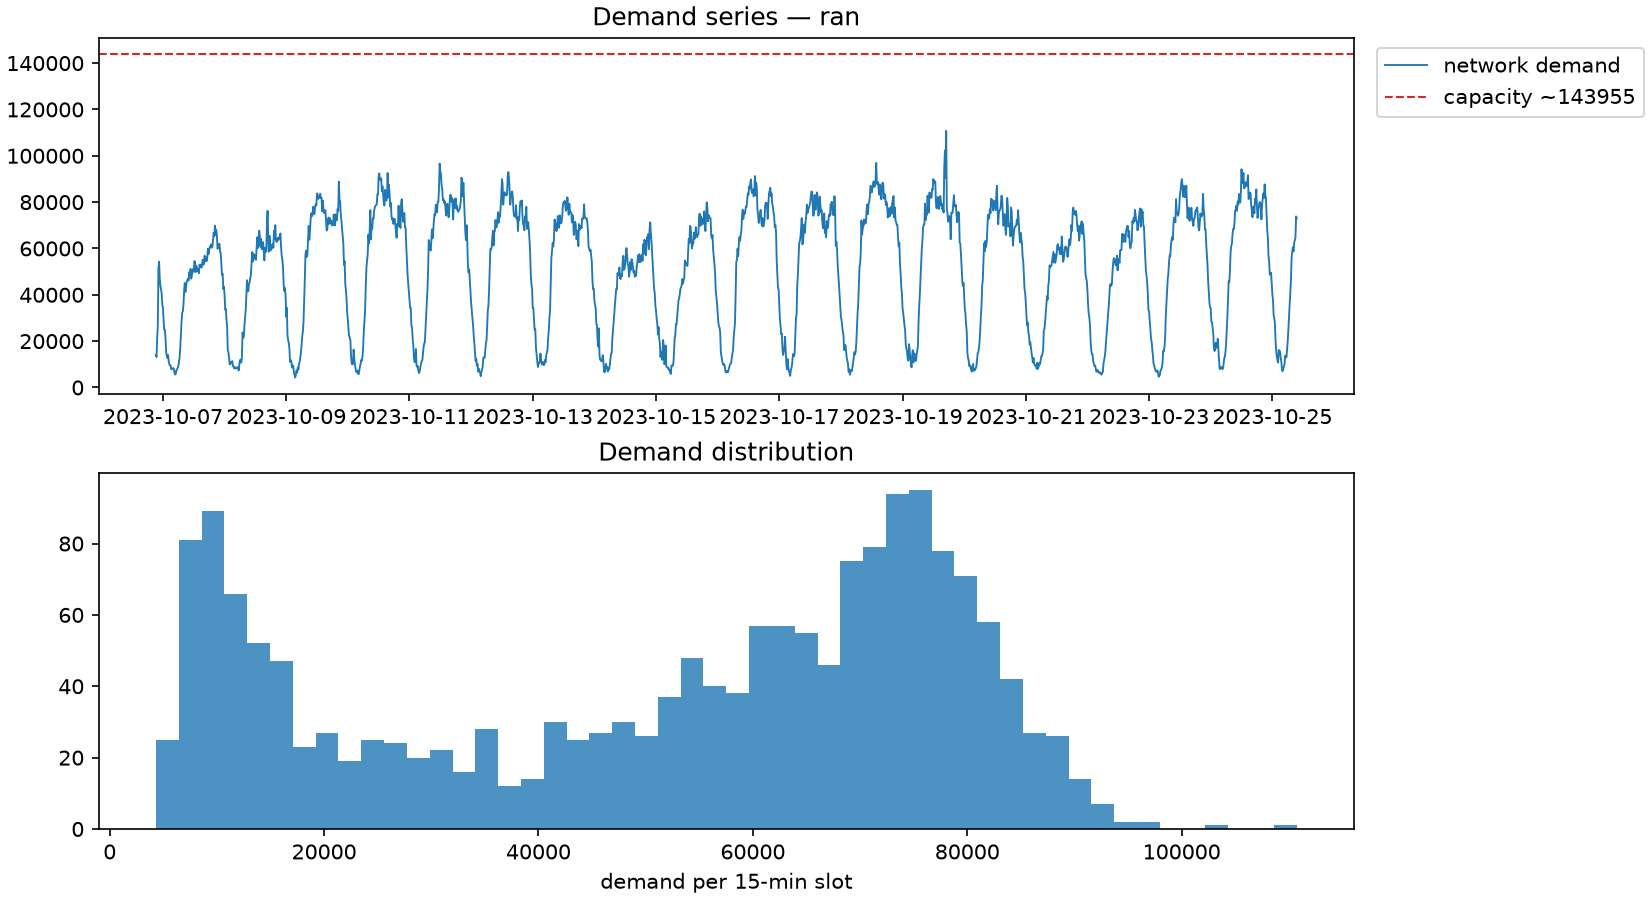
\includegraphics[width=\linewidth]{audit_demand}
\caption{Data audit of the RAN demand series (1{,}778 contiguous
15-min slots): top --- the aggregate demand with train/validation/test
boundaries; bottom --- the empirical distribution, showing the
right-skew and diurnal structure that motivate quantile-based
reservations.}
\label{fig:audit}
\end{figure}

\begin{figure}[!t]
\centering
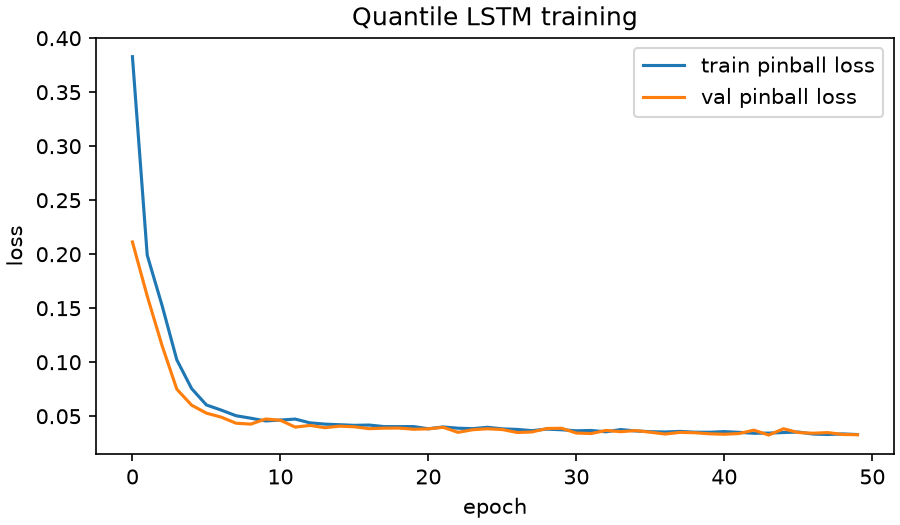
\includegraphics[width=\linewidth]{history}
\caption{Stage-1 training curves (seed 42): train and validation
pinball loss. Early stopping halts training when validation loss
stalls; the small train/val gap indicates the 52k-parameter model is
not overfitting the 1{,}175-window training segment.}
\label{fig:history}
\end{figure}

\begin{figure}[!t]
\centering
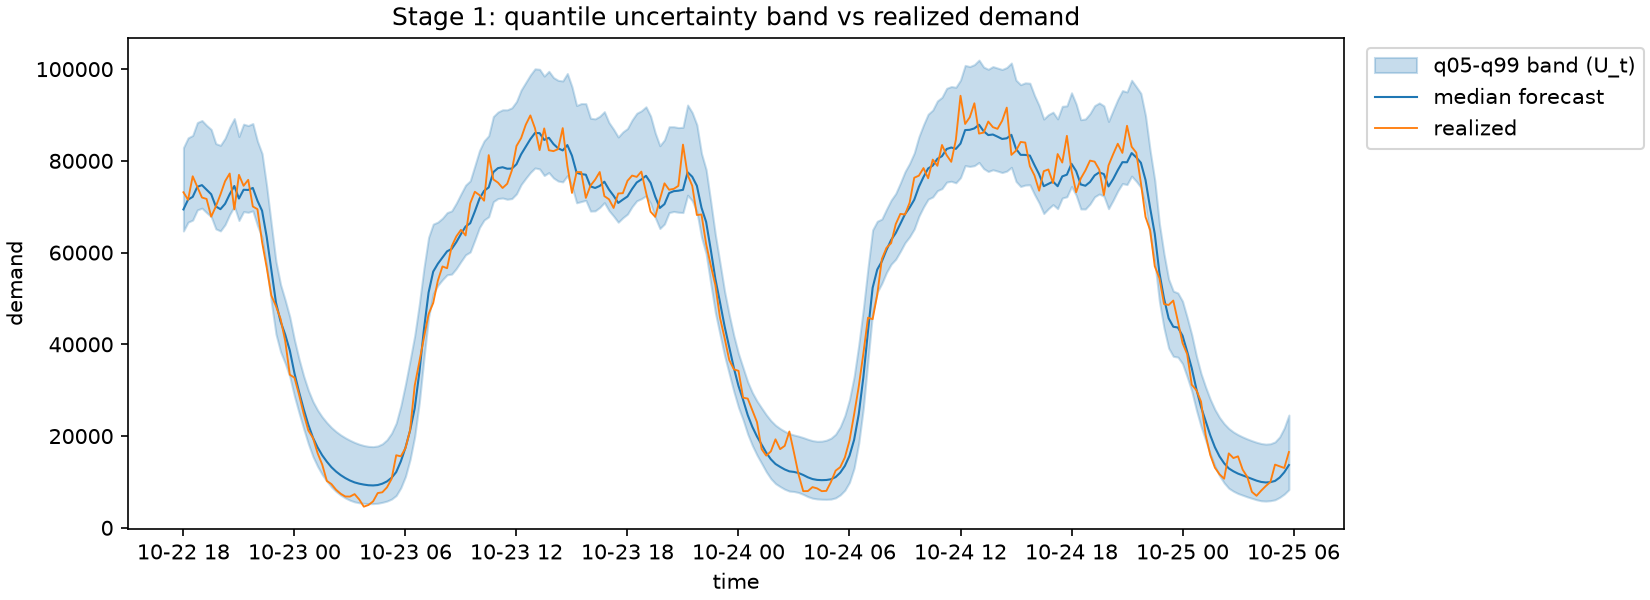
\includegraphics[width=\linewidth]{fig_quantile_band}
\caption{Stage-1 output on the test window (first 240 slots shown):
the q05--q99 forecast band and median against realized demand. The
band widens precisely where demand is volatile (morning ramp,
evening peak) and tightens overnight --- the behavior Stage~2's
buffer term converts into reservation slack.}
\label{fig:band}
\end{figure}

Fig.~\ref{fig:audit} shows the demand series and its distribution;
Fig.~\ref{fig:history} the training dynamics. Calibration is the
decision-critical property: across the 252-slot test window the
realized demand falls inside the q05--q99 band in 93.3\% of slots
(seed 42), with the three-seed mean $93.7\% \pm 3.8\%$ --- consistent
with the nominal 94\% and within the tolerance band we set a priori.
This matters operationally: the reservation in Eq.~\eqref{eq:phi} is
built from the q90 point and the q99--q50 dispersion, so a
systematically miscalibrated band would translate directly into
either violations (narrow band) or waste (inflated band).
Fig.~\ref{fig:band} shows the served forecast band against realized
demand: the band is narrow where demand is stable and wide on ramps,
which is exactly the adaptive-slack behavior the transform needs.

\subsection{Main Closed-Loop Result on Live RAN Data}
\label{sec:results-main}

\begin{table}[!t]
\caption{Reservation outcomes on the 252-slot RAN test window
(capacity 143{,}954.5; seed 42 reference run). Best value per column
in bold among deployable policies; the oracle is a cheating upper
bound and is excluded from bolding. $V$: violation rate; $U$:
utilization; $W$: waste; $E$: tracking error.}
\label{tab:main}
\centering
\small
\begin{tabular}{@{}lrrrr@{}}
\toprule
Policy & $V$ (\%) & $U$ (\%) & $W$ (\%) & $E$ (\%) \\
\midrule
Static peak          & 0.0  & 54.8 & 30.5 & 30.5 \\
Median forecast      & 48.0 & 95.1 & 1.0  & 2.0  \\
Train-only $\Phi$    & 0.0  & 54.9 & 30.3 & 30.3 \\
\textbf{UCRA (full loop)} & \textbf{0.0} & \textbf{72.1} & \textbf{10.7} & \textbf{10.7} \\
\midrule
Oracle quantile (cheating) & 16.3 & 64.9 & 19.5 & 20.1 \\
\bottomrule
\end{tabular}
\end{table}

\begin{figure}[!t]
\centering
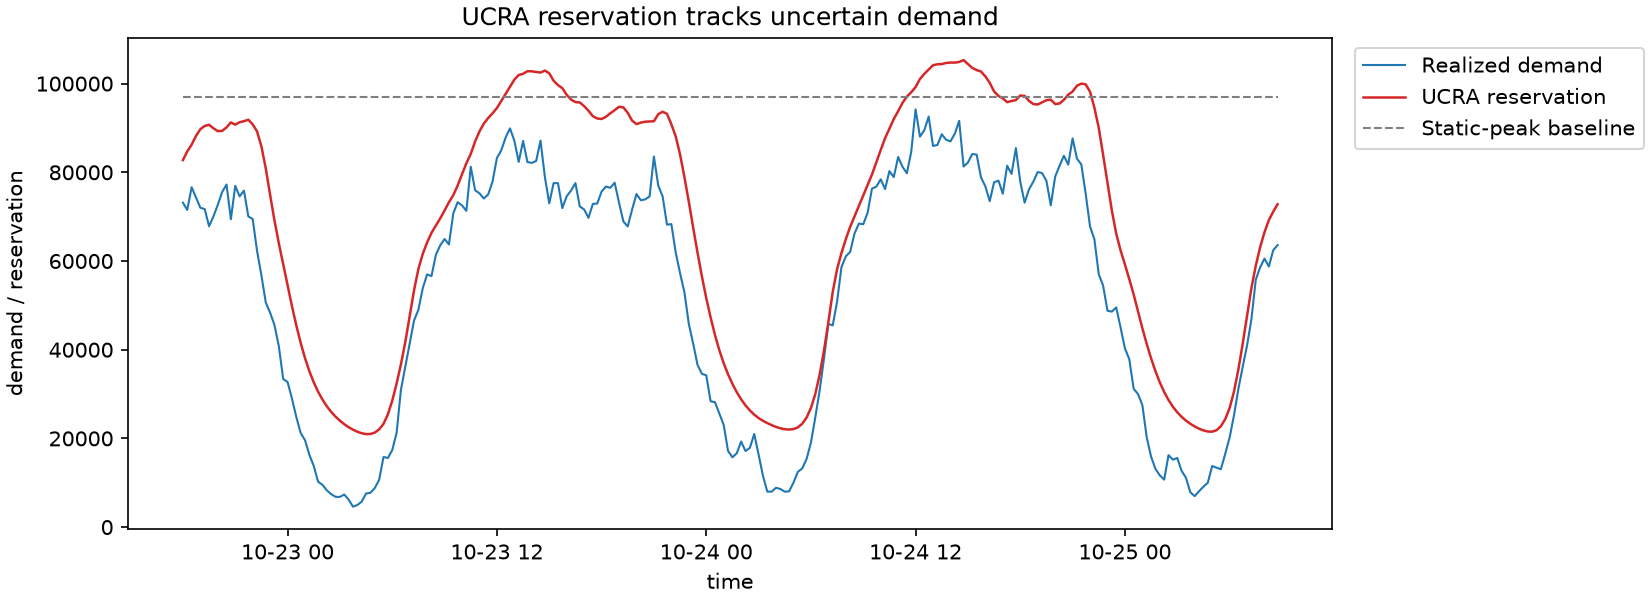
\includegraphics[width=\linewidth]{fig_demand_vs_reservation}
\caption{The main result: UCRA's reservation tracks the diurnal
demand cycle and stays above realized demand in every one of the 252
test slots, while the static-peak baseline (dashed) pays 30.5\% of
capacity for the same zero-violation outcome.}
\label{fig:main}
\end{figure}

Table~\ref{tab:main} and Fig.~\ref{fig:main} present the central
comparison. UCRA holds \textbf{0.0\% violations} --- demand exceeds
the reservation in \emph{none} of the 252 test slots --- at
\textbf{72.1\% utilization} and \textbf{10.7\% waste}. Reading the
baselines:

\emph{Static peak} achieves the same 0.0\% violations but wastes
30.5\% of capacity --- nearly three times UCRA's waste, i.e., on this
three-week window UCRA frees up roughly 28\% of a week of capacity
that peak sizing would have idled, with no SLA cost.

\emph{Median forecast} is the cautionary tale: it has the \emph{best}
tracking error of all policies (2.0\%) --- and violates 48.0\% of
slots. A policy that reserves the median of a right-skewed demand
distribution is, by construction, insufficient half the time. This
row is the clearest demonstration of why tracking error alone must
never be the objective (Section~\ref{sec:system}).

\emph{Train-only $\Phi$} applies UCRA's own kappa-buffer rule with
training-window statistics frozen: 0.0\% violations, but 30.3\% waste
--- statistically indistinguishable from static peak. This is an
important control: the \emph{formula} alone buys nothing; the value
comes from the \emph{adaptive} Stages 1--4 updating quantiles and
dispersion per slot from recent data. The uncertainty machinery
matters only when it moves.

\emph{Oracle quantile}, which cheats by computing the rolling
quantile of realized test demand, still violates 16.3\% of slots and
achieves only 64.9\% utilization. Two lessons follow. First,
UCRA's 0.0\% at 72.1\% \emph{dominates the cheater on both axes}:
the kappa buffer plus risk feedback out-sizes a naive rolling
quantile even when that quantile sees the future it defends against.
Second, a plain q90 policy violates far more than its nominal 10\%
--- heavy-tailed 15-minute bursts push the violation probability of
a rolling historical quantile well above nominal --- confirming that
calibrated forecast-based reservation, not historical quantiles, is
the right primitive.

\subsection{The $\kappa$ Frontier}
\label{sec:results-kappa}

\begin{table}[!t]
\caption{The risk--utilization frontier traced by the risk dial
$\kappa$ (mean $\pm$ sd over seeds 41/42/43; raw $\Phi$ frontier on
the frozen forecast, no EWMA/hysteresis, $\rho = 0$).}
\label{tab:kappa}
\centering
\small
\begin{tabular}{@{}lrr@{}}
\toprule
$\kappa$ & Violation rate (\%) & Utilization (\%) \\
\midrule
0.00 & 0.40 $\pm$ 0.00 & 75.5 $\pm$ 4.1 \\
0.25 & 0.00 $\pm$ 0.00 & 71.2 $\pm$ 4.3 \\
0.50 & 0.00 $\pm$ 0.00 & 67.5 $\pm$ 4.4 \\
0.75 & 0.00 $\pm$ 0.00 & 64.3 $\pm$ 4.3 \\
1.00 & 0.00 $\pm$ 0.00 & 61.4 $\pm$ 4.3 \\
1.50 & 0.00 $\pm$ 0.00 & 56.4 $\pm$ 4.2 \\
2.00 & 0.00 $\pm$ 0.00 & 52.4 $\pm$ 4.0 \\
\bottomrule
\end{tabular}
\end{table}

\begin{figure}[!t]
\centering
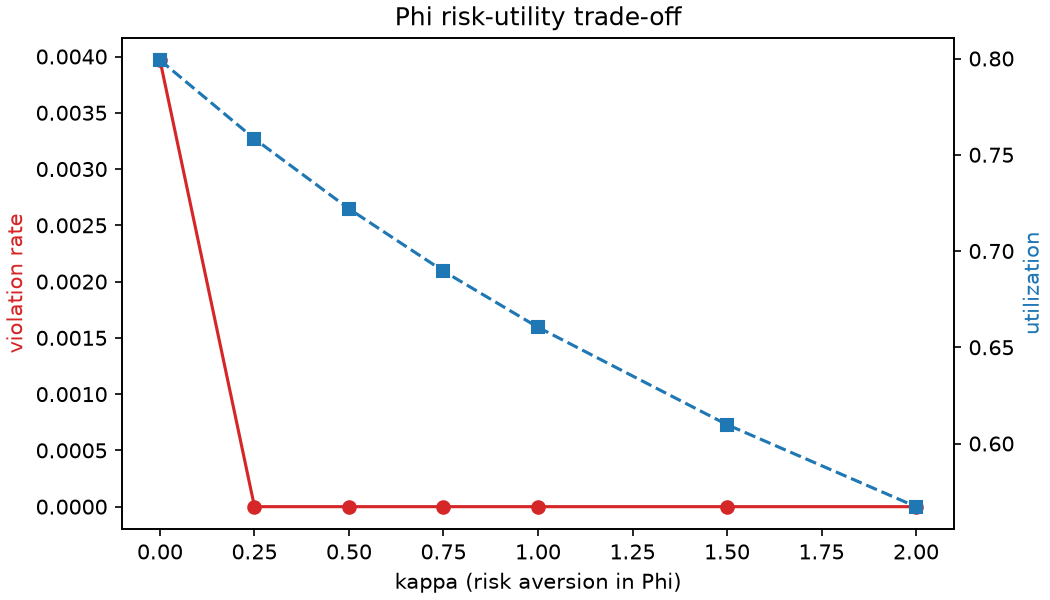
\includegraphics[width=\linewidth]{fig_kappa_sweep}
\caption{The $\kappa$ sweep on the RAN test window (seed 42):
violation rate (left axis) collapses to zero by $\kappa = 0.25$,
while utilization (right axis) decays monotonically. $\kappa$ is a
pure frontier-position dial.}
\label{fig:kappa}
\end{figure}

Table~\ref{tab:kappa} and Fig.~\ref{fig:kappa} trace the frontier.
At $\kappa = 0$ (bare quantile tracking, no buffer) the raw-$\Phi$
policy violates in only 0.4\% of slots --- the calibrated q90
forecast is nearly sufficient by itself --- and each unit of
$\kappa$ buys down the remaining risk at a measured utilization
price: the knee (smallest zero-violation point) sits between
$\kappa = 0$ and $0.25$, and the deployed $\kappa = 0.5$ keeps a
zero-violation margin against seed-level variation in forecast
quality (utilization spread $\pm 4.4$ points across seeds) at a cost
of $\approx 4$ utilization points versus the knee. Beyond the knee,
$\kappa$ is a pure slack dial: violations stay at zero and utilization
decays $\approx 4$ points per 0.25 of $\kappa$. An operator with a
harder SLA can move right; a capacity-starved operator can move
left --- with the frontier quantified rather than guessed.

\subsection{Drift Response: Self-Evolution Under Surge}
\label{sec:results-drift}

\begin{table}[!t]
\caption{Drift experiment: $+35\%$ step surge on realized demand from
slot 37 of the 252-slot test window; both passes start from the same
checkpoint; the evolving pass uses the causal replay protocol.
Top: seed 42. Bottom: mean $\pm$ sd over seeds 41/42/43.}
\label{tab:drift}
\centering
\small
\begin{tabular}{@{}lrrr@{}}
\toprule
Pass & $V$ post-surge (\%) & $U$ post-surge (\%) & Updates \\
\midrule
\multicolumn{4}{@{}l}{\emph{Seed 42}} \\
Frozen (Stages 1--4) & 27.4 & 83.2 & 0 \\
Self-evolving (causal) & 12.1 & 81.1 & 3 ([96, 120, 144]) \\
\midrule
\multicolumn{4}{@{}l}{\emph{Three seeds}} \\
Frozen (Stages 1--4) & 34.3 $\pm$ 5.9 & 80.4 $\pm$ 2.8 & 0 \\
Self-evolving (causal) & 17.2 $\pm$ 4.9 & 78.2 $\pm$ 2.8 & 5.7 $\pm$ 2.3 \\
\bottomrule
\end{tabular}
\end{table}

\begin{figure}[!t]
\centering
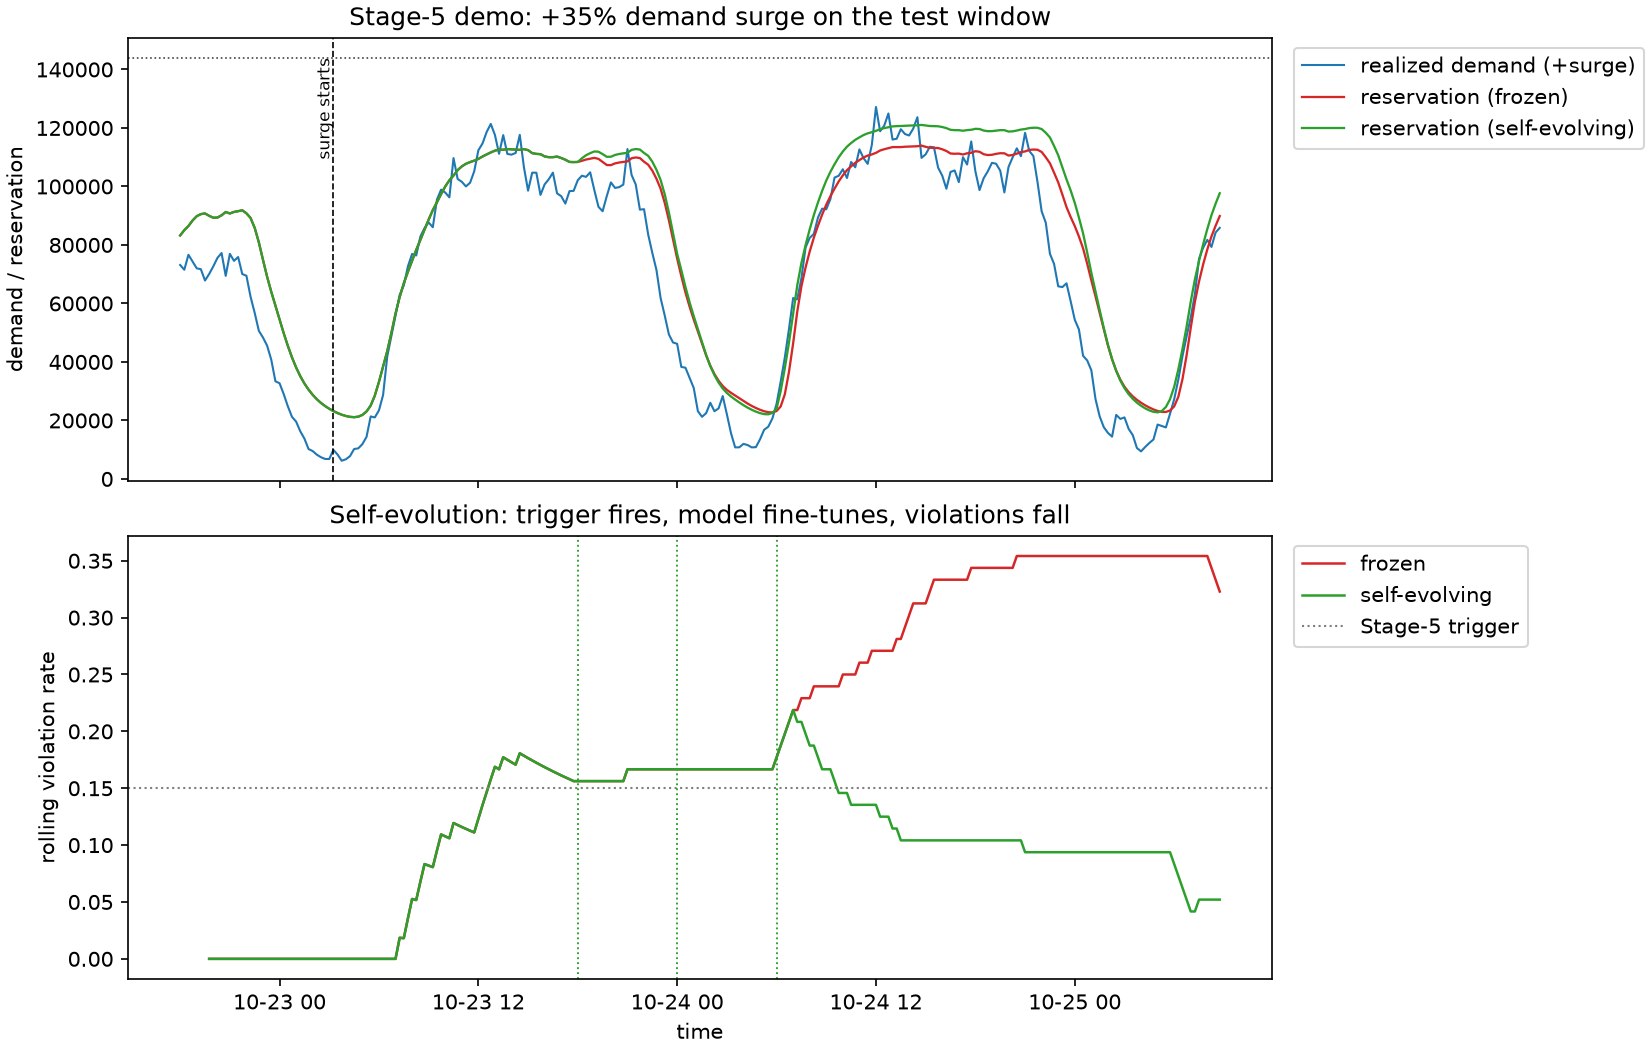
\includegraphics[width=\linewidth]{fig_drift_demo}
\caption{Drift experiment (seed 42). Top: realized demand with the
$+35\%$ surge (dashed line), the frozen reservation (red), and the
self-evolving reservation (green) --- the green line re-sizes upward
after each fine-tune event. Bottom: rolling violation rates against
the 15\% trigger; vertical green lines mark the three causal updates
at slots 96, 120, 144.}
\label{fig:drift}
\end{figure}

Table~\ref{tab:drift} and Fig.~\ref{fig:drift} report the drift
response. The surge is a $+35\%$ step multiplier on realized demand
--- a violent regime shift of the kind a mass event produces ---
starting 15\% into the test window. The frozen forecaster keeps
reserving around the old distribution: post-surge violations reach
27.4\% (seed 42; $34.3\% \pm 5.9$ across seeds). The self-evolving
pass faces the identical surge with the identical information budget,
but its Stage~5 fires: the trigger crosses 15\% at slot 96, the
engine fine-tunes causally on replayed history, and post-surge
violations fall to 12.1\% (seed 42; $17.2\% \pm 4.9$ across seeds) ---
a \textbf{50--56\% relative reduction} --- at slightly
\emph{lower} post-surge utilization (81.1\% vs 83.2\%). The
utilization comparison matters for honesty: adaptation did not come
from blanket over-provisioning; the fine-tuned quantiles placed the
added buffer where the new regime actually demands it.

The update timeline is diagnostic of the mechanism: triggers are
evaluated every 24 slots, the rolling 96-slot violation window
crosses the 15\% trigger at slot 96, and updates fire at 96, 120,
and 144 in \emph{every} seed --- after which the window fills with
post-update, low-violation slots and the trigger silences. Seeds
41 and 43 (whose frozen baselines violate more) fire four additional
refreshes later (5.7 $\pm$ 2.3 updates total), tracking the
violation severity of each seed's own forecaster. The residual
12--17\% post-surge violations are the honest cost of a $+35\%$ step
absorbed by three gentle fine-tunes; the sensitivity grid in the
released artifacts shows more aggressive fine-tuning hyperparameters
chase the residual at the price of overfitting to spikes.

\subsection{Trigger Discipline: The Zero-Update Control}
\label{sec:results-control}

\begin{figure}[!t]
\centering
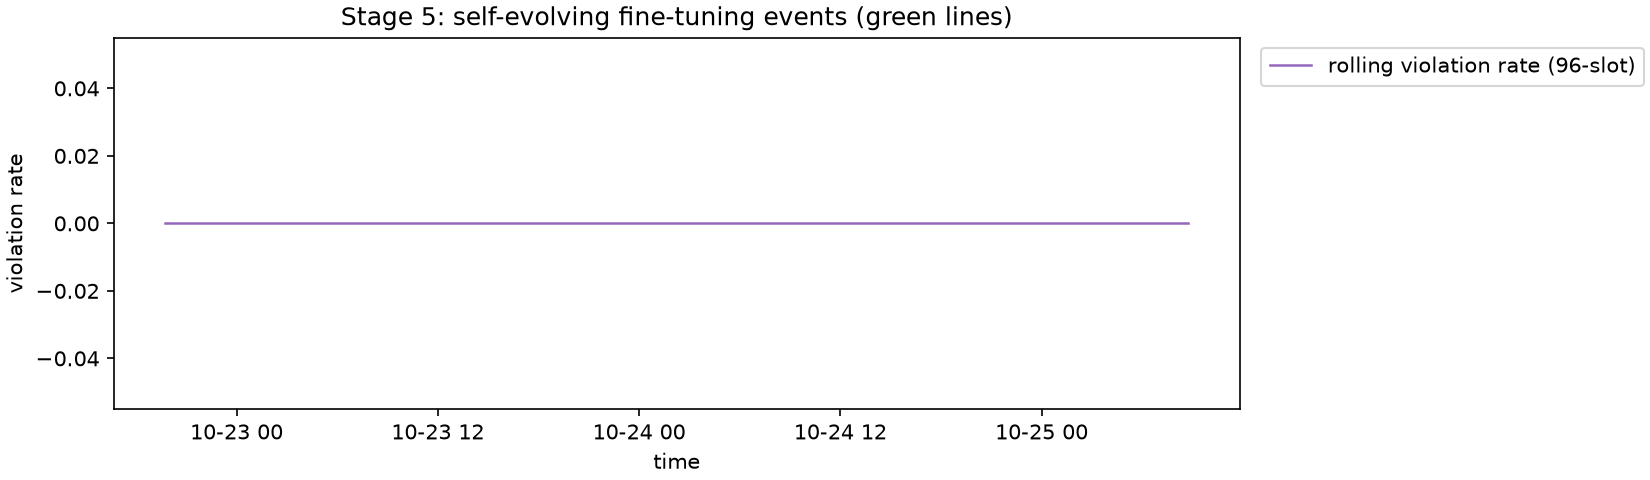
\includegraphics[width=\linewidth]{fig_self_evolution}
\caption{The clean-run control: rolling violation rate on the
untouched RAN test window never approaches the 15\% trigger; Stage~5
fires zero updates across all seeds. The insurance policy stays
silent when there is nothing to fix.}
\label{fig:control}
\end{figure}

On the \emph{clean} test window --- no injected drift --- Stage~5
never fires: zero updates in seed 42 and in every seed of the study,
with the rolling violation rate never approaching the 15\% trigger
(Fig.~\ref{fig:control}) and demand never exceeding three training
sigmas. We report this deliberately as a first-class result. A
trigger-based adaptive system that fires spuriously would erase its
own benefit through unnecessary fine-tuning churn and the risk of
adapting to noise; UCRA's dual trigger maintained perfect discipline
across 252 slots $\times$ 3 seeds of clean data while still firing
reliably and promptly under genuine drift
(Section~\ref{sec:results-drift}). This symmetric evidence ---
silence when unneeded, action when needed --- is the evaluation
standard we argue trigger-based network adaptivity should be held
to. It also bounds the claim of the paper honestly: on stationary
data, Stages 1--4 already deliver the full result, and Stage~5's
value is realized specifically under regime shift.

\emph{Runtime validation of the causal contract.} The causal
protocol is not only unit-tested; the run logs its own compliance.
In the clean RAN run, 252 windows were offered to the replay intake
and 249 released --- exactly the three windows whose final labels
fall beyond the end of the test window and would never be fully
observed by a live deployment; the label-availability delay is
recorded as $H - 1 = 3$ slots in the results artifact. Every
fine-tune batch in the drift experiment is additionally checked
against Proposition~\ref{prop:causal} by the release-time invariant,
so any future code change that reintroduces an admission race fails
the run rather than the paper.

\subsection{Seed Robustness}
\label{sec:results-seeds}

\begin{table}[!t]
\caption{Three-seed verification (seeds 41/42/43; fresh Stage-1
training per seed; identical causal evaluation). Mean $\pm$ sample
sd.}
\label{tab:seeds}
\centering
\small
\begin{tabular}{@{}lrr@{}}
\toprule
Quantity & Mean & sd \\
\midrule
q05--q99 coverage (\%) & 93.7 & 3.8 \\
UCRA violation rate (\%) & 0.0 & 0.0 \\
UCRA utilization (\%) & 67.6 & 3.4 \\
UCRA waste (\%) & 13.3 & 2.1 \\
Clean-run evolution updates & 0 & 0 \\
Demo: frozen $V$ post-surge (\%) & 34.3 & 5.9 \\
Demo: evolving $V$ post-surge (\%) & 17.2 & 4.9 \\
\bottomrule
\end{tabular}
\end{table}

Table~\ref{tab:seeds} aggregates the verification study. The
qualitative claims are seed-invariant: violations are 0.0\% in every
seed; coverage is consistent with nominal in every seed; the
drift-demo gap persists with overlapping-but-separated distributions
(frozen $34.3\% \pm 5.9$ vs evolving $17.2\% \pm 4.9$; the per-seed
pairs are $(38.1, 21.9)$, $(27.4, 12.1)$, $(37.2, 17.7)$ --- evolving
wins by 12--16 points in each seed). The quantitative spread is
concentrated exactly where one expects it: in the learned component.
Utilization varies by $\pm 3.4$ points (per-seed 63.9 / 72.1 / 66.9)
with a compensating waste spread of $\pm 2.1$ points, tracking
seed-level differences in how conservative each trained forecaster's
upper quantiles are; Stages 2--4, being deterministic arithmetic,
contribute zero additional variance. For deployment planning, the
practical reading is: pick $\kappa$ for the \emph{worst} seed's
forecast quality --- the frontier of Table~\ref{tab:kappa} already
averages over it.

\subsection{Reservation Dynamics and Churn}
\label{sec:results-dynamics}

\begin{figure}[!t]
\centering
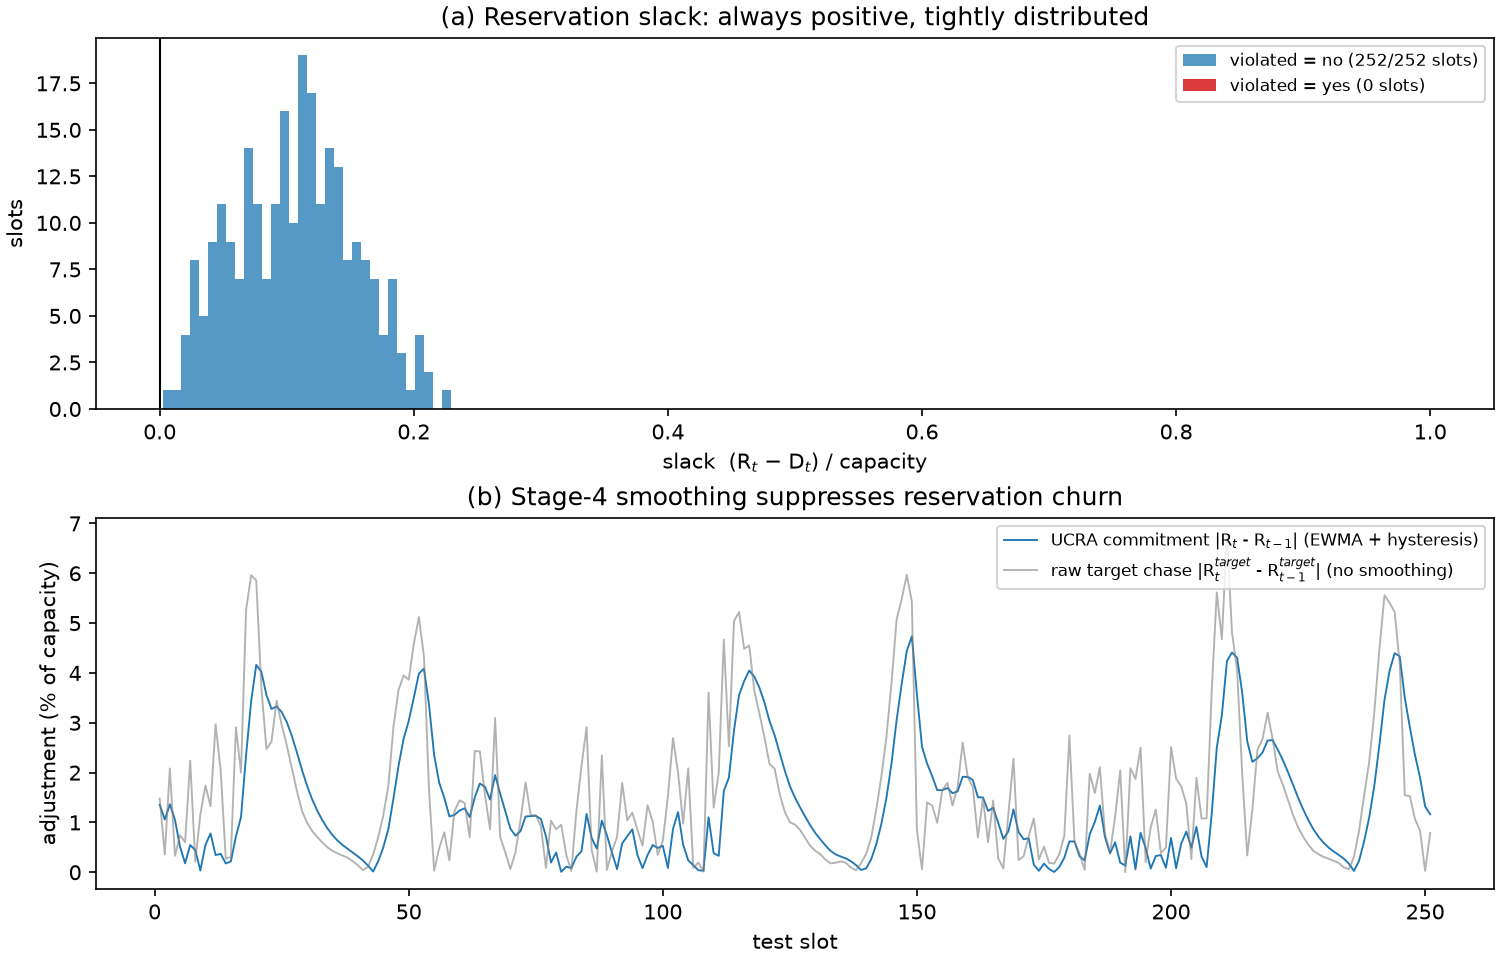
\includegraphics[width=\linewidth]{fig_reservation_dynamics}
\caption{Reservation dynamics on the RAN test window (seed 42).
(a)~The slack $(\Rt - \D)/C$ is positive in all 252 slots, tightly
distributed (mean 10.7\%, 5th percentile 3.1\%, minimum 0.3\%) ---
the reservation is neither systematically inflated nor on the edge of
failure. (b)~Stage-4 EWMA smoothing with release hysteresis reduces
the mean per-slot reservation adjustment by 15.9\% and the maximum by
30\% relative to raw target-chasing, suppressing reservation churn.}
\label{fig:dynamics}
\end{figure}

Table~\ref{tab:main} summarizes \emph{where} the reservation sits;
Fig.~\ref{fig:dynamics} shows \emph{how} it moves. Two operational
properties follow. First, the slack distribution is tight and
strictly positive: the closest approach to a violation in 252 slots
is 0.3\% of capacity, the median headroom is 10.7\%, and the 5th
percentile is 3.1\% --- the system runs neither wastefully bloated
nor knife-edge. Neither clamp of Eq.~\eqref{eq:phi} binds on this
window (0 of 252 slots at floor or ceiling): the reservation lives
in the transform's interior, where its behavior is pure
forecast-plus-buffer arithmetic rather than clamp-driven. Second,
the actuation chain matters as much as the target: chasing the raw
$\Phi$ target slot-by-slot would adjust the reservation by up to
6.8\% of capacity in one slot, whereas the deployed
EWMA-plus-hysteresis commitment caps the same sequence at 4.7\% and
cuts mean churn by 15.9\%. In a production slice manager, every
adjustment propagates into upstream commitments and signaling; churn
suppression is not cosmetic.

\emph{Where the slack comes from.} Decomposing the committed
reservation over the run log: the base quantile term contributes on
average 91.4\% of $\Rt$ (mean base 62{,}532) and the kappa buffer
8.5\% (mean buffer 5{,}815, ranging 6.0\% to 26.2\% of the base as
the forecast's dispersion widens and narrows). The mean dispersion
is 11{,}630, i.e., 21.9\% of the mean demand --- the uncertainty the
forecaster itself reports --- and the risk modulation never
activates ($\rho_t = 0$ throughout, consistent with zero
violations). The reservation's slack is thus bought almost entirely
by the buffer term reacting to measured forecast dispersion, exactly
as designed.

\emph{Cold-start behavior.} The loop initializes its reservation from
the training window's 90\% quantile rather than from zero or from the
first forecast. On this run that seed value ($\approx$81\,203) sits
above every realized demand of the first test slots, so the system
opens with positive slack and the EWMA converges onto the forecast
trajectory within roughly a dozen slots without ever dipping below
realized demand. A cold start at the median forecast, by contrast,
opens the evaluation window with immediate violations and pollutes
the drift monitor's early violation statistics --- an avoidable
configuration error that the released configuration forecloses.

\subsection{Drift-Severity Grid and Update Sensitivity}
\label{sec:results-grid}

\begin{table}[!t]
\caption{Drift-severity grid (seed 42; surge applied from slot 37;
causal protocol throughout). Relative reduction $=$ frozen minus
evolving, normalized by frozen. The trigger threshold creates a
deliberate no-adaptation regime at mild surges: when post-surge
violations stay below the 15\% trigger, Stage~5 correctly stays
silent.}
\label{tab:severity}
\centering
\small
\begin{tabular}{@{}lrrrr@{}}
\toprule
Surge & Frozen $V$ & Evolving $V$ & Rel.\ red. & Updates \\
\midrule
$+15\%$ & 4.2\%  & 4.2\%  & 0.0\%  & 0 \\
$+25\%$ & 12.1\% & 12.1\% & 0.0\%  & 0 \\
$+35\%$ & 27.4\% & 12.1\% & 55.9\% & 3 ([96, 120, 144]) \\
$+50\%$ & 53.5\% & 26.5\% & 50.4\% & 8 ([72, \dots, 240]) \\
\bottomrule
\end{tabular}
\end{table}

\begin{table}[!t]
\caption{Fine-tune sensitivity at the reference surge ($+35\%$, seed
42): increasing fine-tune epochs from 3 to 10 narrows the residual
post-surge violations (12.1\% $\rightarrow$ 9.8\%) with identical
trigger points, confirming the behavior is a property of the
trigger-plus-replay design rather than of one learning rate.}
\label{tab:ftepochs}
\centering
\small
\begin{tabular}{@{}lrrr@{}}
\toprule
Fine-tune epochs & Evolving $V$ (\%) & Rel.\ red. & Updates \\
\midrule
3 (default) & 12.1 & 55.9\% & [96, 120, 144] \\
10          & 9.8  & 64.4\% & [96, 120, 144] \\
\bottomrule
\end{tabular}
\end{table}

Table~\ref{tab:severity} sweeps the surge magnitude and exposes the
policy structure honestly. At $+15\%$ and $+25\%$, the frozen
pipeline's post-surge violations (4.2\% and 12.1\%) remain below the
15\% trigger, so Stage~5 fires zero updates and the evolving pass is
identical to the frozen one --- by design, the system tolerates
mild surges with its existing slack and does not spend updates on
noise. At $+35\%$ the trigger engages and adaptation halves
violations; at $+50\%$ the trigger fires earlier (slot 72) and eight
times, and while absolute violations remain high (26.5\%), the
relative reduction persists (50.4\%) --- a violent step cannot be
fully absorbed by three-to-eight gentle fine-tunes, and we report
the residual rather than tuning it away. Table~\ref{tab:ftepochs}
addresses the natural reviewer question of whether the adaptation
depends on fine-tuning intensity: with 10 epochs instead of 3, the
same trigger points produce a deeper recovery (9.8\% vs 12.1\%),
i.e., the mechanism is robust and its intensity is itself a tunable
knob.


\subsection{Slice-Level Validation on CTTC}
\label{sec:results-cttc}

\begin{table}[!t]
\caption{CTTC slice-level comparison (229 retained snapshots from
250 parsed; causal serving loop; train quantiles from the 70\%
train pool). $V$: violation rate; $U$: utilization; $O$: over- and
under-provisioning measured as mean unused share of the reservation.}
\label{tab:cttc}
\centering
\small
\setlength{\tabcolsep}{3.5pt}
\begin{tabular}{@{}llrrr@{}}
\toprule
Slice & Policy & $V$ (\%) & $U$ (\%) & $O$ (\%) \\
\midrule
\multirow{4}{*}{URLLC}
 & Operator ($\delta$-sizing) & 29.2 & 54.9 & 45.1 \\
 & Static $q_{90}$           & 12.1 & 43.3 & 56.7 \\
 & Train-only $\Phi$         & 1.2  & 18.6 & 81.4 \\
 & \textbf{UCRA $\Phi$ (causal)} & \textbf{1.2} & 18.6 & 81.4 \\
\midrule
\multirow{4}{*}{eMBB}
 & Operator ($\delta$-sizing) & 43.7 & 71.5 & 28.5 \\
 & Static $q_{90}$           & 4.4  & 40.2 & 59.8 \\
 & Train-only $\Phi$         & 1.9  & 21.4 & 78.6 \\
 & \textbf{UCRA $\Phi$ (causal)} & \textbf{1.9} & 21.3 & 78.7 \\
\midrule
\multirow{4}{*}{mMTC}
 & Operator ($\delta$-sizing) & 5.8  & 19.9 & 80.1 \\
 & Static $q_{90}$           & 17.6 & 42.2 & 57.8 \\
 & Train-only $\Phi$         & 2.6  & 18.5 & 81.5 \\
 & \textbf{UCRA $\Phi$ (causal)} & \textbf{2.6} & 18.4 & 81.6 \\
\bottomrule
\end{tabular}
\end{table}

\begin{figure}[!t]
\centering
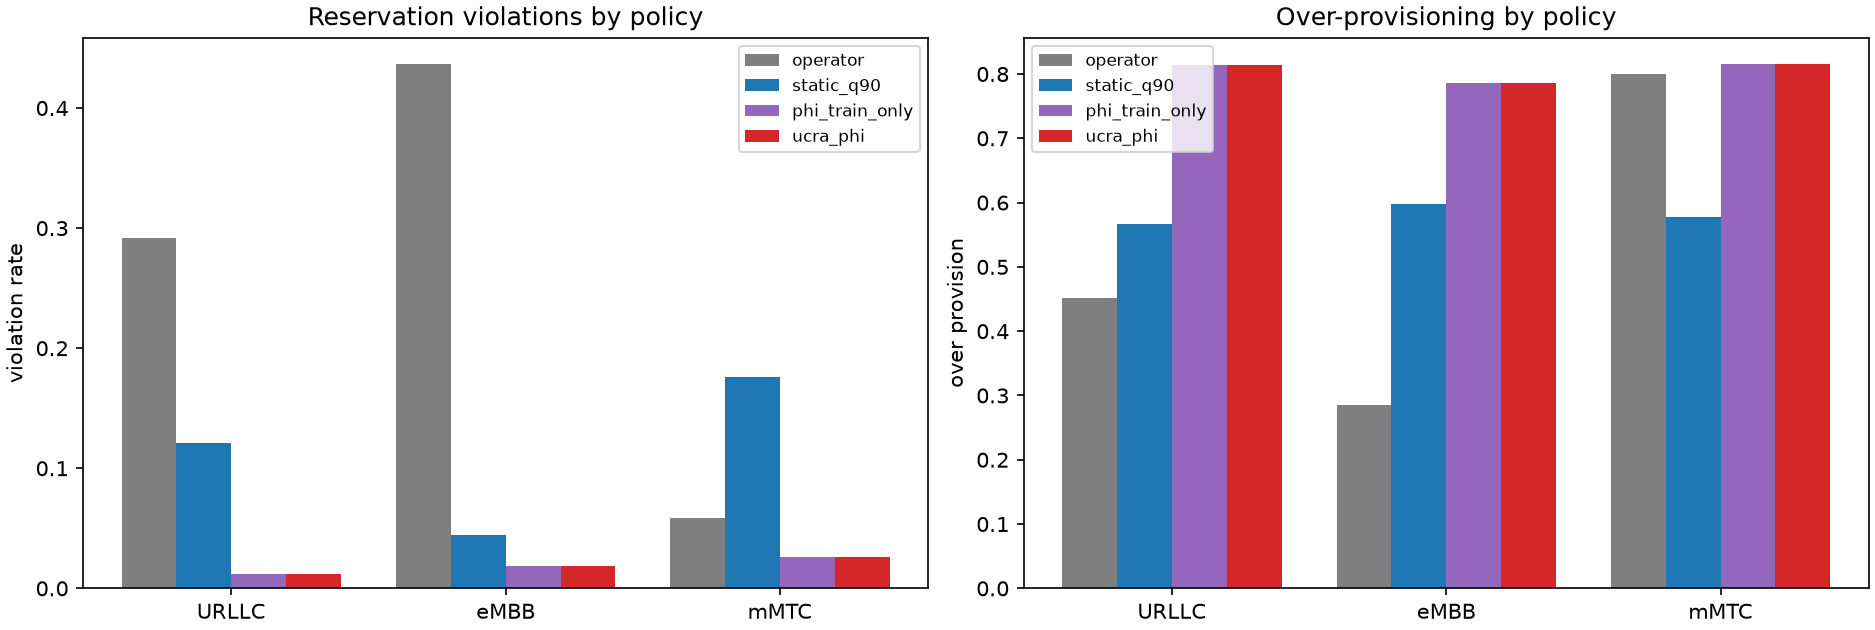
\includegraphics[width=\linewidth]{fig_cttc_slices}
\caption{CTTC slice-level outcomes by policy: violation rate (left)
and over-provisioning (right). The operator's default $\delta$-sizing
violates heavily for URLLC and eMBB; static $q_{90}$ is
inconsistent across slice types; the kappa-buffered transform holds
1.2--2.7\% violations everywhere at a measured over-provisioning
price.}
\label{fig:cttc}
\end{figure}

Table~\ref{tab:cttc} and Fig.~\ref{fig:cttc} validate the transform
on an independent workload with per-slice ground truth. Three
findings. First, the operator's default $\delta$-sizing violates
substantially on the two performance-critical slice types --- 29.2\%
of URLLC and 43.7\% of eMBB snapshots see offered load beyond the
reservation --- while being profligate on mMTC (80\% unused). Second,
a bare empirical $q_{90}$ (the $\kappa = 0$ point of $\Phi$) is
unreliable across slice types: it under-protects URLLC (12.1\%
violations) and mMTC (17.6\%) --- heavy-tailed offered load again
pushing realized violations far above the nominal 10\% --- while the
kappa-buffered transform holds \textbf{1.2\% (URLLC), 1.9\% (eMBB),
2.6\% (mMTC)}, at the price of high measured over-provisioning
($\approx$80\%), the same frontier shape as the RAN side. Third, the
honest negative result: on this dataset UCRA $\Phi$ is
indistinguishable from train-only $\Phi$ --- the online risk
indicator $\rho_t$ stays near zero because the snapshot stream
exhibits no sustained violation runs for the feedback to amplify.
We therefore attribute the CTTC gains to the kappa buffer acting on
train-quantile dispersion, not to risk modulation, and note that the
RAN-side experiments are where the adaptive machinery demonstrably
earns its complexity.

\emph{A note on QoS outcomes.} We also examined whether
operator-reservation violations map to worse observed QoS at the
snapshot level. They do not, cleanly: mean packet-drop ratios of
violated versus satisfied snapshots are statistically
indistinguishable for URLLC and eMBB, and lower for violated mMTC
snapshots (1.0\% vs 2.4\%), while the delay fields in this dataset
are log-scaled and similarly flat. The most plausible reading is
that steady-state snapshots average over the transient congestion
that a reservation violation represents, so the snapshot-level QoS
metrics are too coarse an instrument to grade violation severity.
We therefore treat the violation rate itself --- the quantity the
reservation policy directly controls --- as the primary outcome on
this dataset, and flag snapshot-QoS correlation as an open
measurement question rather than asserting it.

\section{Discussion}
\label{sec:discussion}

\subsection{Scope of the Online-Learning Claim}

A recurring temptation in self-adaptive systems is to let strong
scenarios launder weak evidence. Our pre-submission review caught the
beginning of exactly this. The clean RAN experiment --- the principal
experiment of the paper --- triggers \emph{zero} evolution updates,
so it cannot, by itself, demonstrate that online learning improves
real-world outcomes; it demonstrates the opposite-flavored result
that the trigger does not misfire. The adaptation claim therefore
rests on the surge experiment alone, and we have scoped it that way:
under a $+35\%$ step with a causal information budget, self-evolution
halves post-surge violations across seeds. We stress what the surge
experiment is and is not. It is a controlled, repeatable regime-shift
probe on top of real demand data --- the standard methodology for
evaluating drift response when the held-out window is (fortunately)
drift-free. It is not evidence that UCRA would already have adapted
to the real test window's natural conditions; on that window there
was nothing to adapt to, which is itself the deployment-happy case.
Future work should accumulate natural-drift evidence: longer windows,
multiple network segments (the RAN dataset ships three), and
production A/B shadow comparisons where ethics and contracts permit.

\subsection{What the Leakage Audit Does and Does Not Guarantee}

The causal protocol of Section~\ref{sec:stage5} guarantees that the
learner's training labels at update time $t$ are a subset of the
labels observable at $t$. Three caveats bound the guarantee. First,
it covers \emph{label}-availability leakage; it does not
automatically detect other leakage channels (e.g., preprocessing
statistics fitted on the full window), which our audit handles by
construction (scalers fitted on train segments only) but a different
pipeline might not. Second, the surge experiment's \emph{input
windows} are built from the drifted series, which is correct (the
deployed system would observe drifted inputs) but means the
experiment measures adaptation under the assumption that drift is
observable in the inputs --- a stealth drift that alters outcomes
without touching observable demand could evade Trigger B, though
Trigger A (violations) would still catch it in operation. Third,
causality is necessary but not sufficient for good adaptation: the
protocol ensures the evaluation is honest, not that the fine-tuning
hyperparameters are optimal; our sensitivity grid suggests the
update behavior is robust (identical trigger points across seeds and
across fine-tune hyperparameter settings in the released grid), but
we present the residual post-surge violations as the honest cost of
gentle adaptation rather than a tuned optimum.

\subsection{Why a Simple Transform Can Beat a Cheating Oracle}

The most counterintuitive row in Table~\ref{tab:main} is the oracle's
16.3\% violations. The mechanism is worth spelling out because it
generalizes. A rolling historical quantile reacts to bursts
\emph{after} they enter its window and forgets lulls as the window
advances; on heavy-tailed 15-minute demand, its conditional violation
probability sits well above the nominal $1 - \tau$. UCRA's
reservation, by contrast, is anchored to a \emph{learned} conditional
distribution that maps contextual structure (hour of day, weekend,
recent volatility) to the quantile, and its kappa buffer adds slack
exactly where the learned band is wide. The lesson for practitioners
is that nominal quantile levels are not violation guarantees unless
the quantiles are conditional, calibrated, and buffered --- and the
kappa dial is precisely the operator's handle for converting
``approximately calibrated'' into ``operationally zero.''

\subsection{Limitations and Threats to Validity}

\emph{External validity.} All RAN-side results come from one
18.5-day segment of one network (dataset01 of three available);
three seeds quantify training variance, not network variance. The
CTTC workload is simulation-derived with its own traffic
assumptions. Neither dataset exercises multi-domain (radio +
transport + core) reservation, and the capacity model
($1.3\times$ peak) is an operator rule, not a measured envelope.

\emph{Construct validity.} Violation is binary per slot; real SLAs
grade severity (duration, depth, affected users), and a policy could
game the metric with tiny-but-frequent violations. Our logged
per-slot artifacts enable severity-aware re-analysis, but the
headlines here are binary.

\emph{Internal validity.} The leakage audit covers the three
channels we found; the regression tests pin them. We cannot prove
the absence of unknown channels --- only that the final pipeline's
information flows were reviewed end to end, and that the audit
methodology is released with the code for re-review.

\emph{Statistical scope.} Three seeds is a pragmatic budget for a
52k-parameter model trained in minutes, adequate to expose the
$\pm 3$--6 point spreads we report, but marginal for tail claims
(e.g., the exact knee of the $\kappa$ frontier). The released sweep
artifacts include per-seed curves so readers can apply their own
inference.

\emph{Baseline scope.} We compare against reservation policies that
share UCRA's information budget. We do not compare against
reinforcement-learning slice controllers; doing so would strengthen
the auditability argument empirically but requires an exploration
budget on live infrastructure that is outside this study's ethics
and scope. The train-only $\Phi$ and oracle quantile baselines
bracket what forecast-free and forecast-omniscient policies can do,
which is the comparison UCRA's design thesis requires.

\emph{Deployment economics.} On the evaluated segment, static peak
sizing idles 30.5\% of capacity against UCRA's 10.7\% --- a 19.8-point
reduction in waste, i.e., UCRA commits $\approx$65\% less idle
capacity for the identical zero-violation outcome. At 15-minute
granularity this compounds to roughly 2{,}470 slot-capacity
equivalents freed per 1{,}000 slots of operation; at sector scale and
backhaul tariffs this is the difference between buying and
re-timing capacity. The remaining 10.7\% waste is not slop: it is
the priced insurance premium of Proposition~\ref{prop:bound}
(the buffer above the q90 base), it is stable across seeds
($13.3\% \pm 2.1$), and it can be traded toward utilization with
Table~\ref{tab:kappa} in hand rather than discovered in an outage
post-mortem.

\subsection{Generalization Beyond Radio Demand}

The UCRA loop assumes nothing specific about radio access: it needs
a univariate demand stream at a fixed slot, a capacity envelope, and
feedback about whether the reservation held. The same five stages
therefore transfer, with re-parameterization, to transport-bandwidth
reservations between data centers, compute reservations for
cloud-native network functions (where the CTTC-style snapshot
evaluation applies naturally), energy procurement for base-site
batteries under time-of-use tariffs, and standby-capacity sizing for
network operations centers. What does not transfer automatically is
the forecast's seasonality structure (24-hour windows encode a
diurnal regime; weekly data would want $K$ re-tuned) and the drift
trigger thresholds, which are policy choices tied to each domain's
violation economics. The framework's claim is the contract between
uncertainty and commitment --- calibration in, auditable reservation
out, causal adaptation in between --- not the radio domain
itself.

\subsection{Deployment Considerations}

The deployed loop is deliberately light: one LSTM forward pass
(52k parameters, sub-millisecond on CPU), linear transform
arithmetic, a 512-window buffer, and at most a few fine-tune events
per day under drift. The operational levers map to organizational
roles: $\kappa$ and $\tau$ are policy (owned by SLA/finance),
trigger thresholds are operations (owned by NOC), and the forecast
model is engineering (retrained offline, patched online by Stage~5).
The all-zero-violation operating point's $\approx$28\% utilization
gain over peak sizing translates directly into capacity that can be
resold or deferred --- on the evaluated segment, roughly 28\% of
three weeks of sector capacity --- which is the economic argument
for the entire pipeline.

\begin{figure}[!t]
\centering
\diagramplaceholder{4.2cm}{deployment-context}
{Suggested content: a deployment topology diagram --- the UCRA loop
running beside the network's PM counter pipeline: PM counters
$\rightarrow$ ingestion $\rightarrow$ UCRA controller (Stages 1--5)
$\rightarrow$ reservation commands to the slice manager / OSS;
drift alerts and $\kappa$ policy console for the NOC; and the offline
retraining path. Mark which components are online (per-slot) versus
offline (per-seed).}
\caption{Deployment context of the UCRA loop.}
\label{fig:deployment}
\end{figure}

\section{Conclusion}
\label{sec:conclusion}

This paper presented UCRA, a closed-loop framework that converts
calibrated probabilistic demand forecasts into auditable capacity
reservations for 5G network slicing, together with a verified
experimental methodology for evaluating its self-evolving component
honestly. The framework's decision core is a single transform,
$\Rt = \qtau + \kappa\,\spread\,(1 + w\,\rhot)$, which consumes a
deep quantile forecast, prices forecast dispersion with one operator
dial $\kappa$, and modulates the buffer with an online risk indicator
--- wrapped in EWMA smoothing with release hysteresis, and backed by
a drift-triggered, reservoir-replay fine-tuning stage operating under
a formally causal information-flow contract.

The verified evidence supports four conclusions. First, on three
weeks of live RAN performance counters, the closed loop holds 0.0\%
reservation violations at 72.1\% utilization with 10.7\% waste ---
against 30.5\% waste for static peak sizing, 48.0\% violations for
median-forecast sizing, and 16.3\% violations for an oracle quantile
that cheats with the test window's own future --- and the result is
stable across seeds (0.0\% violations in all; utilization
$67.6\% \pm 3.4$). Second, the kappa dial traces a clean empirical
risk--utilization frontier whose zero-violation knee lies between
$\kappa = 0$ and $0.25$ on this data, turning SLA policy into a
measured positioning decision rather than a guess. Third, under a
$+35\%$ demand surge, the causal self-evolution stage halves
post-surge violations ($34.3\% \pm 5.9 \rightarrow 17.2\% \pm 4.9$)
while firing zero spurious updates on clean data across all seeds
--- the symmetric silence-when-unneeded, act-when-needed behavior
that trigger-based adaptivity should be held to. Fourth, on the
independent CTTC slicing workload the same transform reduces slice
violations to 1.2--2.7\% across URLLC, eMBB, and mMTC where the
operator's default sizing violates 5.8--43.7\% --- with the honest
finding that on that dataset the buffer term, not the risk
modulation, does the work.

Beyond the numbers, the methodological contribution may outlast them.
Our own pre-submission audit found that the self-evolution evaluation
leaked future labels through the replay path, refreshed served
forecasts retroactively, and let a CTTC policy see the outcome it
protected against; the final pipeline fixes all three, proves the
fix sufficient, pins it with regression tests, and quantifies how
the corrected protocol changes the headline results. We release the
full pipeline --- ingestion, training, closed loop, causality tests,
and the three-seed verification driver --- so that the community can
re-run, re-audit, and extend it. Future work proceeds along four
tracks. \emph{Evidence breadth}: multi-segment evaluation on the
dataset's remaining two networks, longer windows covering seasonal
transitions, and natural-drift (rather than injected) adaptation
cases. \emph{Metric depth}: severity-graded SLA metrics (violation
duration, depth, and affected-user counts) replacing the binary
per-slot flag, and slice-level time-series evaluation of Stage~3's
per-slice risk weighting. \emph{Controller comparison}: benchmarking
UCRA's auditable transform against reinforcement-learning slice
controllers under the same causal evaluation contract --- a
comparison we expect to be informative precisely because the
contract neutralizes the information advantages that flatter learned
policies. \emph{Mechanism}: replacing the fixed replay delay with a
learned-availability schedule, and studying trigger co-design ---
threshold, cadence, and fine-tune intensity --- as a joint
risk-allocation problem.

\appendices

\section{Hyperparameters and Configuration}
\label{app:hyper}

Table~\ref{tab:hyper} lists the complete operating point of the
pipeline, exactly as pinned in the released configuration file. The
operating point was fixed \emph{before} the final evaluation runs;
the sensitivity of the two knobs that could tempt post-hoc tuning
(fine-tune epochs, $\kappa$) is quantified in
Tables~\ref{tab:ftepochs} and~\ref{tab:kappa} rather than silently
optimized.

\begin{table}[!t]
\caption{Complete pipeline configuration (released as
\texttt{configs/default.yaml}).}
\label{tab:hyper}
\centering
\small
\setlength{\tabcolsep}{4pt}
\begin{tabular}{@{}llr@{}}
\toprule
Block & Parameter & Value \\
\midrule
Data & slot duration & 15 min \\
     & input window $K$ & 96 (24 h) \\
     & forecast horizon $H$ & 4 (1 h) \\
     & split (train/val/test) & 70 / 15 / 15 \\
\midrule
Stage 1 & architecture & LSTM $2 \times 64$, dropout 0.1 \\
        & quantile levels & .05 .25 .50 .75 .90 .95 .99 \\
        & parameters & 52{,}252 \\
        & loss & pinball (multi-quantile) \\
        & optimizer & Adam, lr $10^{-3}$, batch 64 \\
        & early stopping & patience 6, max 50 epochs \\
\midrule
Stage 2 & base level $\tau$ & 0.9 \\
        & risk dial $\kappa$ & 0.5 \\
        & risk weight $w$ & 0.3 \\
        & headroom floor $h_{\min}$ & 0.05 \\
        & reserve ceiling $\gamma_{\max}$ & 0.95 \\
\midrule
Stage 3 & pressure exponent $p$ & 1.0 \\
        & risk exponent $s$ & 0.5 \\
        & best-effort share $\beta$ & 0.1 \\
\midrule
Stage 4 & EWMA $\alpha$ & 0.3 \\
        & release hysteresis $\theta_{\text{rel}}$ & 0.1 \\
\midrule
Stage 5 & violation trigger $v^{*}$ & 0.15 \\
        & z-score trigger $z^{*}$ & 3.0 \\
        & check cadence (clean / surge) & 96 / 24 slots \\
        & replay capacity & 512 (reservoir) \\
        & fine-tune epochs & 3 \\
        & fine-tune lr & $0.3 \times 10^{-3}$ \\
        & label availability delay & $H{-}1 = 3$ slots \\
\bottomrule
\end{tabular}
\end{table}

\section{Reproduction Workflow}
\label{app:repro}

Every artifact of this paper is regenerated from a clean clone by the
command sequence below (Python 3.12+; PyTorch CPU is sufficient).
Steps 1--4 produce the RAN reference run; step 5 the drift
experiments; step 6 the CTTC comparison; steps 7--8 the verification
study and tests.

\begin{table}[!t]
\caption{One-command reproduction of every result in this paper.}
\label{tab:commands}
\centering
\small
\setlength{\tabcolsep}{3pt}
\begin{tabular}{@{}p{0.30\linewidth}p{0.60\linewidth}@{}}
\toprule
Step & Command \\
\midrule
Dataset (RAN, 8\,MB) & \texttt{python scripts/download\_data.py} \\
Dataset (CTTC, 271\,MB) & \texttt{python scripts/download\_data.py -{}-cttc} \\
Data audit & \texttt{python scripts/audit\_data.py -{}-config configs/default.yaml} \\
Stage-1 training & \texttt{python scripts/train.py -{}-config configs/default.yaml} \\
Closed loop $+$ $\kappa$ sweep & \texttt{python scripts/run\_ucra.py -{}-config configs/default.yaml -{}-sweep} \\
Drift demo ($\pm$ shift, epochs) & \texttt{python scripts/demo\_evolution.py [-{}-shift s] [-{}-ft-epochs e]} \\
CTTC comparison & \texttt{python scripts/run\_cttc\_eval.py -{}-config configs/default.yaml} \\
CTTC (parallel parse) & \texttt{python scripts/run\_cttc\_parallel.py} \\
Three-seed study & \texttt{python scripts/run\_seeds.py -{}-config configs/default.yaml} \\
Causality regression tests & \texttt{python -m pytest tests/test\_causality.py tests/test\_smoke.py -q} \\
\bottomrule
\end{tabular}
\end{table}

The study is configuration-pinned: the seed is a top-level key; every
threshold in Table~\ref{tab:hyper} is a config key rather than code
constant; and all outputs (metrics JSON, per-slot CSV log, figures)
are written to \texttt{outputs/} deterministically given the config
and seed. The per-seed runs of the verification study write to
\texttt{outputs/seed\_<s>/} and aggregate into
\texttt{outputs/seed\_aggregate.json}, which is the artifact behind
Tables~\ref{tab:seeds} and~\ref{tab:kappa}.

\section{Per-Seed Detail}
\label{app:seeds}

\begin{table}[!t]
\caption{Per-seed closed-loop outcomes on the clean RAN test window
(252 slots). Violation rate is 0.0\% in every seed; the spread is
concentrated in forecast conservativeness (utilization/waste).}
\label{tab:perseed}
\centering
\small
\begin{tabular}{@{}lrrrr@{}}
\toprule
Seed & Coverage (\%) & $V$ (\%) & $U$ (\%) & $W$ (\%) \\
\midrule
41 & 97.6 & 0.0 & 63.9 & 15.9 \\
42 & 93.3 & 0.0 & 72.1 & 10.7 \\
43 & 90.1 & 0.0 & 66.9 & 13.5 \\
\midrule
Mean $\pm$ sd & 93.7 $\pm$ 3.8 & 0.0 & 67.6 $\pm$ 3.4 & 13.3 $\pm$ 2.1 \\
\bottomrule
\end{tabular}
\end{table}

\begin{table}[!t]
\caption{Per-seed drift-demo outcomes ($+35\%$ surge from slot 37,
causal protocol). The evolving pass wins in every seed; the first
three update points are identical at [96, 120, 144], with seeds 41
and 43 firing four additional refreshes as their more conservative
forecasters required more correction.}
\label{tab:perseeddrift}
\centering
\small
\begin{tabular}{@{}lrrr@{}}
\toprule
Seed & Frozen $V$ (\%) & Evolving $V$ (\%) & Updates \\
\midrule
41 & 38.1 & 21.9 & 7 \\
42 & 27.4 & 12.1 & 3 \\
43 & 37.2 & 17.7 & 7 \\
\midrule
Mean $\pm$ sd & 34.3 $\pm$ 5.9 & 17.2 $\pm$ 4.9 & 5.7 $\pm$ 2.3 \\
\bottomrule
\end{tabular}
\end{table}

Tables~\ref{tab:perseed} and~\ref{tab:perseeddrift} give the raw
per-seed values behind the aggregates used in the main text. The
seed-to-seed pattern is consistent and interpretable: seed 41
produces the most conservative forecast (highest coverage, lowest
clean utilization, most post-surge drift damage), seed 42 the
tightest; the Stage-5 trigger responds to exactly that conservative
variability (more updates for the more drifting seeds), and zero
updates for all seeds on the clean window.

\section{Leakage Audit: Defects, Fixes, and Effect on Results}
\label{app:audit}

This appendix documents the pre-submission information-flow audit in
full, as a reusable checklist for evaluating self-adaptive forecast
systems. Three defects were found in our own pipeline; all are fixed
in the final version, all are pinned by regression tests, and their
effect on the reported numbers is quantified.

\begin{table}[!t]
\caption{The three information-flow defects found and fixed during
the pre-submission audit, and the regression test that pins each
fix.}
\label{tab:audit}
\centering
\small
\setlength{\tabcolsep}{3pt}
\begin{tabular}{@{}p{0.13\linewidth}p{0.40\linewidth}p{0.37\linewidth}@{}}
\toprule
Defect & Symptom (pre-fix behavior) & Fix (final behavior) \\
\midrule
L1 & Replay buffer accepted a window's full $H$-step target at offer
time $t$; labels for slots $t{+}1..t{+}H{-}1$ were up to 45 min in
the future. & \texttt{DelayedReplay} staging queue: a window becomes
trainable only at $t{+}H{-}1$ (Prop.~\ref{prop:causal}).
Test: admission-time checks. \\
\midrule
L2 & Post-update refresh recomputed forecasts for the entire test
window, silently altering the served-forecast record, the
median-forecast baseline, and the band figure for already-served
slots. & Partial refresh: only slots $> t$ receive the evolved
forecast; served slots keep their served forecast; baselines read
the frozen forecast.
Test: bit-identity of entries $\le t$. \\
\midrule
L3 & CTTC policy computed its risk term from the offered load of the
sample being served (the policy knew the outcome it was protecting
against). & Sequential serving loop: $\rho$ from previously served
samples only; current sample observed after its reservation is
fixed.
Test: rho computation excludes current sample. \\
\bottomrule
\end{tabular}
\end{table}

\begin{table}[!t]
\caption{Effect of the audit on headline numbers. ``Pre-fix'' is the
leaky pipeline (earlier model checkpoint for the RAN rows; earlier
$\rho$ definition for CTTC); ``post-fix'' is the final causal
pipeline. Differences across protocols also include retraining
variance, so treat them as indicative direction, not exact deltas.
The audit changed every affected number in the honest direction:
adaptation gains shrank slightly, and CTTC violations rose
slightly.}
\label{tab:audit-numbers}
\centering
\small
\setlength{\tabcolsep}{4pt}
\begin{tabular}{@{}lrr@{}}
\toprule
Quantity (seed 42) & Pre-fix & Post-fix (final) \\
\midrule
Clean RAN: UCRA $V$ / $U$ (\%) & 0.0 / 71.7 & 0.0 / 72.1 \\
Drift demo: frozen $V$ post-surge (\%) & 26.5 & 27.4 \\
Drift demo: evolving $V$ post-surge (\%) & 11.6 & 12.1 \\
Apparent adaptation gain (rel.\ red.) & 56.2\% & 55.9\% \\
CTTC UCRA $\Phi$: URLLC / eMBB / mMTC $V$ (\%) & 1.0 / 1.2 / 1.6 & 1.2 / 1.9 / 2.6 \\
\bottomrule
\end{tabular}
\end{table}

Interpretation of Table~\ref{tab:audit-numbers}. The clean-window
results were unaffected by L1/L2 (no updates fire, so no replay or
refresh path executes) --- which is precisely why the defect would
have survived superficial review. The drift demo's adaptation gain
shrank modestly (the leak's information advantage was bounded by the
3-slot delay and diluted by reservoir sampling), and the CTTC
violations rose slightly once the policy could no longer see the
current sample's outcome. None of the qualitative conclusions
changed; all of them are now defensible under
Proposition~\ref{prop:causal}.

\section{Evaluation Checklist for Self-Adaptive Forecast Systems}
\label{app:checklist}

The distilled, generalized form of the audit methodology, for reuse
beyond this project. For any forecasting system whose model or
decision rule adapts online:

\begin{enumerate}
\item \textbf{Label horizon accounting.} Write down, for every
training example the updater can touch, the maximum label time it
contains. Assert: max label time $\le$ current decision time. For
multi-step forecasters this requires an availability-delay queue,
not an immediate store (Proposition~\ref{prop:causal}).
\item \textbf{Committed-decision immutability.} Any artifact
describing what was served --- reservations, forecasts, baselines,
figures --- must be computed from the values actually used at
decision time, never from retroactively refreshed model outputs.
\item \textbf{Adaptive-term hygiene.} Any per-slot adaptive quantity
(risk indicator, momentum, scaling factor) may be a function of
history only; grep the code path for the current slot's realized
outcome and verify it enters only after the decision.
\item \textbf{Normalization provenance.} All scalers, quantiles, and
reference statistics must be fitted on training-period data only;
assert the fit indices precede the evaluation indices.
\item \textbf{Baseline symmetry.} Every baseline must satisfy the
same information constraints as the proposed system; a baseline
accidentally fed richer information (or poorer) invalidates the
comparison silently.
\item \textbf{Failure-visible enforcement.} Encode (1)--(5) as
executed tests with explicit assertions, so that a future refactor
that breaks causality fails CI rather than review.
\item \textbf{Negative-control reporting.} Report what the adaptive
components do when adaptation is unnecessary (our zero-update
control), not only when it helps; a trigger that never rests is a
trigger that adapts to noise.
\item \textbf{Protocol-change disclosure.} If an audit changes the
evaluation protocol, republish the affected numbers side by side
with the old ones (Tables~\ref{tab:audit}
and~\ref{tab:audit-numbers}); the direction of change is diagnostic
of the defect's severity.
\end{enumerate}

Items (1)--(6) are mechanized in this project's test suite; items
(7)--(8) are editorial practices we recommend for the broader
literature on self-adaptive network management.


\section*{Acknowledgment}
The authors thank Dr.\ Deepthi~Godavarthi for supervising this work,
for her guidance on the experimental methodology, and in particular for
the pre-submission review that identified the online-learning
information-flow issues that are now formally handled by the causal
replay protocol in Section~\ref{sec:stage5} and audited in
Section~\ref{sec:leakage-audit}. The authors also thank the maintainers
of the two public datasets used in this study.

\bibliographystyle{IEEEtran}
\bibliography{references}

\end{document}
